%!TEX TS-program = pdflatex
% dissertation.tex -- main dissertation file
%
% Wisconsin dissertation template
% Copyright (c) 2008-2009 William C. Benton.  All rights reserved.
%
% This program can redistributed and/or modified under the terms
% of the LaTeX Project Public License Distributed from CTAN
% archives in directory macros/latex/base/lppl.txt; either
% version 1 of the License, or (at your option) any later version.
%
% This program includes other software that is licensed under the
% terms of the LPPL and the Perl Artistic License; see README for details.
%
% You, the user, still hold the copyright to any document you produce
% with this software (like your dissertation).
%

%%% You'll want ``oneside'' for the deposit version, but probably not for any versions that don't need to meet the UW requirements
\documentclass[12pt,oneside,letterpaper]{memoir}

% preamble.tex -- packages to include
%
% Wisconsin dissertation template
% Copyright (c) 2008 William C. Benton.  All rights reserved.
%
% This program can redistributed and/or modified under the terms
% of the LaTeX Project Public License Distributed from CTAN
% archives in directory macros/latex/base/lppl.txt; either
% version 1 of the License, or (at your option) any later version.
%
% This program includes other software that is licensed under the
% terms of the LPPL and the Perl Artistic License; see README for details.
%
% You, the user, still hold the copyright to any document you produce
% with this software (like your dissertation).


%% You probably need appendix, if you want appendices
\IfFileExists{appendix.sty}{%
\usepackage{appendix}%
}{}

%% the spacing in memoir is weird, you'll need to use this
\DisemulatePackage{setspace}
\usepackage[doublespacing]{setspace}
\setstretch{2}
%% geometry package to help with margins on title page
\usepackage{geometry}

%% List setup; the ``hanglist`` environment will allow you to have
%% nicely-typeset enumerated lists (i.e. with the numbers hanging in
%% the margins).  You need at least version 2.1 of enumitem.sty.  If
%% you don't have enumitem installed at all, hanglist will just be an
%% alias for enumerate.
\IfFileExists{enumitem.sty}{%
\usepackage[loadonly]{enumitem}[2007/06/30]%
\newlist{hanglist}{enumerate}{1}% 
\setlist[hanglist]{label=\arabic*.}%
\setlist[hanglist,1]{leftmargin=0pt}%
}{%
\newenvironment{hanglist}{\begin{enumerate}}{\end{enumerate}}%
}

%% Comment out any of these that you don't want
\usepackage{amssymb}
\usepackage{amsmath}
\usepackage{amsthm}
%\usepackage{theorem}
\usepackage{hyperref}
\usepackage{listings}
\usepackage{titletoc}
\usepackage{tocloft}

% \usepackage[super,comma,numbers,sectionbib,sort&compress]{natbib} % docs: %http://merkel.zoneo.net/Latex/natbib.php

\usepackage[authoryear,round,sectionbib,sort&compress]{natbib}

\usepackage{chapterbib}
\usepackage{longtable}
\newcommand\nomen[2]{#1 & #2 \\}

\usepackage{listings}
\usepackage{xcolor}

\lstdefinestyle{sharpc}{language=[Sharp]C, frame=lr, rulecolor=\color{blue!80!black}}

\usepackage{placeins} % had [section]
\usepackage{float}

\IfFileExists{mathpartir.sty}{%
\usepackage{mathpartir}%
}{}

%%%%% LISTINGS package and setup
\IfFileExists{listings.sty}{%
\usepackage{listings}%
}{}


%% Get rid of ugly borders around PDF hyperlinks (e.g. for cross-references, bib entries, or URLs)
\hypersetup{pdfborder = 0 0 0}

%% You want microtype.
\IfFileExists{microtype.sty}{%
\usepackage[protrusion=true,expansion=true]{microtype}%
}{}

%\pagestyle{thesisdraft}

% Surround parts of graphics with box
\usepackage{boxedminipage}

%% booktabs (thx to Nate Rosenblum for bringing this beautiful package
%% to my attention)
\IfFileExists{booktabs.sty}{%
\usepackage{booktabs}%
}{}

% This is now the recommended way for checking for PDFLaTeX:
\usepackage{ifpdf}

%% Avoid ugly "Type 3" fonts
\usepackage{lmodern}
\usepackage[LY1]{fontenc}

%% Substitute your favorite serif and sans fonts here....
\IfFileExists{tgpagella.sty}{%
% TeX Gyre pagella, like Palatino
\usepackage{tgpagella}%
}{}

\usepackage[LY1]{eulervm}

\ifpdf
\usepackage[pdftex]{graphicx}
\else
\usepackage{graphicx}
\fi


% DJB additions
\usepackage{grffile}   
\usepackage{rotating}  % Enables sideway figure and captions
\usepackage[labelfont=bf]{caption} % Bolds the Figure x.x part of the caption


\usepackage{makeidx}
\makeindex


{\theoremstyle{plain}
\newtheorem{thm}{Theorem}[chapter]
\newtheorem{cor}[thm]{Corollary}
\newtheorem{define}[thm]{Definition}
\newtheorem{exmpl}[thm]{Example}
}
{\theoremstyle{remark}
\newtheorem{rmk}[thm]{Remark}
}

\newtheoremstyle{customsty1}
{3pt}%
{3pt}%
{}% --- body font
{}% --- indent amount
{\bfseries}% --- Theorem head font
{:}% --- Punctuation after head
{.5em}% --- space after head
{}% --- theorem head spec (can be left empty, meaning 'normal')

% Define 'newtheorems' that use ``customsty1''
{\theoremstyle{customsty1}
}

%%%%DCG EDITS

\usepackage{blindtext}
\usepackage[CaptionAfterwards]{fltpage}
\usepackage{lipsum}
\usepackage{pdfpages}
\usepackage{setspace}
%\usepackage{newclude}


%%% NB: the ``deposit'' chapter- and page- styles should conform to UW
%%% requirements.  If you are producing a pretty version of your
%%% dissertation for web use later, you will certainly want to make
%%% your own chapter and page styles.

\makechapterstyle{deposit}{%
  \renewcommand{\chapterheadstart}{}
  \renewcommand{\printchaptername}{}
  \renewcommand{\chapternamenum}{}
  \renewcommand{\printchapternum}{\center\bfseries Chapter \thechapter}
  \renewcommand{\afterchapternum}{}
  \renewcommand{\printchaptertitle}[1]{%
  \center\Large\scshape\MakeLowercase{##1}}
  \renewcommand{\afterchaptertitle}{%
  \vskip\onelineskip}
}

\usepackage{titlesec}
\usepackage{rotating}
\usepackage{numprint}

%Edited by DCG
% hide the section numbers 
%\renewcommand\thesection{} 
%\setsecindent{-3em}


\titleformat*{\section}{\normalfont\bfseries}

%DCG changed from runin to hang and changed spacing between titles
\titleformat{\section}[hang]{\normalfont\bfseries}{\thesection.}{12pt}{}
\titleformat{\subsection}[hang]{\normalfont\bfseries}{\thesubsection.}{12pt}{}
\titleformat{\subsubsection}[runin]{\normalfont\bfseries}{\thesubsubsection.}{12pt}{}

\newcommand*{\mycaption}[2]{\caption[#1]{\textbf{#1.} #2}}
\renewcommand{\bibname}{References}



\makepagestyle{deposit}
 
\makeatletter

\renewcommand{\chaptermark}[1]{\markboth{#1}{}}
\renewcommand{\sectionmark}[1]{\markboth{#1}{}}
 
% No Footers
\makeevenfoot{deposit}{}{}{}
\makeoddfoot{deposit}{}{}{}

% Make the page number always appear in the top right of the page
\makeevenhead{deposit}{\thepage}{}{}
\makeoddhead{deposit}{}{}{\thepage}

\makeatother

%%% set up page numbering for chapter pages to satisfy UW requirements
%%% NB: You will want to delete until the ``SNIP'' mark if you are
%%% making a ``nice'' copy
\copypagestyle{chapter}{plain}
\makeoddfoot{chapter}{}{}{}
\makeevenhead{chapter}{\thepage}{}{}
\makeoddhead{chapter}{}{}{\thepage}
%%% SNIP

%%% bib nonsense
\makeatletter
\newenvironment{wb-bib}[1]{%
  \section{References}
\ifnobibintoc\else 
\phantomsection 
\fi 
\prebibhook
 \begin{bibitemlist}{#1}}{\end{bibitemlist}\postbibhook}

\AtBeginDocument{%
 \@ifpackageloaded{natbib}{% natbib is loaded
  \addtodef{\endthebibliography}{}{\vskip-\lastskip\postbibhook}
    \@ifpackagewith{natbib}{sectionbib}{% with sectionbib option
      \renewcommand{\bibsection}{\@memb@bsec}}%
      {\renewcommand{\bibsection}{\@memb@bchap}}}%
  {}
  \@ifpackagewith{chapterbib}{sectionbib}{%
   \renewcommand{\sectionbib}[2]{}
    \renewcommand{\bibsection}{\@memb@bsec}}{}
}
\makeatother

% defs.tex -- wbepi environment for chapter epigraphs and other useful defs.
%
% Wisconsin dissertation template
% Copyright (c) 2008 William C. Benton.  All rights reserved.
%
% This program can redistributed and/or modified under the terms
% of the LaTeX Project Public License Distributed from CTAN
% archives in directory macros/latex/base/lppl.txt; either
% version 1 of the License, or (at your option) any later version.
%
% This program includes other software that is licensed under the
% terms of the LPPL and the Perl Artistic License; see README for details.
%
% You, the user, still hold the copyright to any document you produce
% with this software (like your dissertation).


%% put lstnewenvironment declarations here, if you're using listings

%% end lstnewenvironment declarations

%% I put convenience definitions that will go in several chapters here

%%%%% begin convenience definitions

\makeatletter
\newcommand{\wb@episource}{}
\newenvironment{wbepi}[1]{\begin{quote}\renewcommand{\wb@episource}{#1}\itshape}{\par\upshape \raggedleft --- \textsc{\wb@episource}\\ \end{quote}}
\makeatother

%%%%% SVN
\IfFileExists{svn-multi.sty}{%
\usepackage{svn-multi}%
%%% Uncomment the second one and comment out the first one if you want
%%% to include subversion revision information in each file.
\newcommand{\vcinfo}{}%
%\newcommand{\vcinfo}{\begin{centering}\fbox{\fbox{\parbox{5in}{Author: \svnauthor\\Revision: \svnfilerev\\Last changed on: \svnfiledate\\URL: \svnkw{HeadURL}}}}\\[1em]\end{centering}}%
}{%
\newcommand{\svnidlong}[4]{}%
\newcommand{\svnfilerev}{}%
\newcommand{\svnauthor}{}%
\newcommand{\svnfiledate}{}%
\newcommand{\svnkw}{}%
\newcommand{\vcinfo}{}%
}

%%%%% end convenience definitions

% thesisdefs.tex

% This is mostly adapted from withesis.cls.  The original copyright
% notice for withesis.cls follows, preceded by two percent signs (%%):

%% withesis.cls
%% LaTeX Style file for the University of Wisconsin-Madison Thesis Format
%% Adapted from the Purdue University Thesis Format
%% Originally by Dave Kraynie
%% Edits by Darrell McCauley
%% Adapted to UW-Madison format by Eric Benedict  (Noted with <EB>)
%% Updated to LaTeX2e by Eric Benedict 24 July 00
%% 
%%=============================================================================
%% Licensed under the Perl Artistic License.
%% see: http://www.ctan.org/tex-archive/help/Catalogue/licenses.artistic.html
%% for more info...
%%=============================================================================

% withesis.cls is available from CTAN.  The modifications to this file
% are also licensed under the Perl Artistic License.

% --wb, 2008

\makeatletter

\newcounter {tocpage}
\newcounter {lofpage}
\newcounter {lotpage}
\newcounter {listofheading}

\newcommand\@thesistitlemedskip{0.25in}
\newcommand\@thesistitlebigskip{0.55in}
\newcommand{\degree}[1]{\gdef\@degree{#1}}
\newcommand{\project}{\gdef\@doctype{A masters project report}}
\newcommand{\prelim}{\gdef\@doctype{A preliminary report}}
\newcommand{\thesis}{\gdef\@doctype{A thesis}}
\newcommand{\dissertation}{\gdef\@doctype{A dissertation}}
\newcommand{\department}[1]{\gdef\@department{(#1)}}
\newcommand{\oralexamdate}[1]{\gdef\@oralexamdate{#1}} 
\newcommand{\committeeone}[1]{\gdef\@committeeone{#1}}
\newcommand{\committeetwo}[1]{\gdef\@committeetwo{#1}}
\newcommand{\committeethree}[1]{\gdef\@committeethree{#1}}
\newcommand{\committeefour}[1]{\gdef\@committeefour{#1}}
\newcommand{\committeefive}[1]{\gdef\@committeefive{#1}}
\newcommand{\committeesix}[1]{\gdef\@committeesix{#1}}
\newcommand{\committeeseven}[1]{\gdef\@committeeseven{#1}}

\newenvironment{titlepage}
 {\@restonecolfalse\if@twocolumn\@restonecoltrue\onecolumn
  \else \newpage \fi \thispagestyle{empty}
% \c@page\z@ -- deleted: count title page in thesis
}{\if@restonecol\twocolumn \else \newpage \fi}

\gdef\@degree{Doctor of Philosophy}    %Default is PhD
\gdef\@doctype{A dissertation}         %Default is dissertation

\gdef\@department{(Electrical Engineering)} % Default is Electical Engineering
\gdef\@oralexamdate{}
\gdef\@committeeone{}
\gdef\@committeetwo{}
\gdef\@committeethree{}
\gdef\@committeefour{}
\gdef\@committeefive{}
\gdef\@committeesix{}
\gdef\@committeeseven{}



\renewcommand{\maketitle}{%
  \begin{titlepage}
%-----------------------------------------------------------------------------
% -- The thesis office doesn't like thanks on title page.  Put it in
% -- the acknowledgments.  This is here so you don't have to change
% -- your titlepage when converting from report style. -> from Purdue, but I
%        left it here since it seems compatible with UW-Madison, Eric
%-----------------------------------------------------------------------------
    \def\thanks##1{\typeout{Warning: `thanks' deleted from thesis titlepage.}}
    \let\footnotesize\small \let\footnoterule\relax \setcounter{page}{1}
 %sets new margins for title page so that committee members can be placed there

   % \vspace*{0.1in}
\begin{SingleSpace}
    \begin{center}
      {\textbf{\expandafter\uppercase\expandafter{\@title}}} \\[\@thesistitlebigskip]
       by \\[\@thesistitlemedskip]
      \@author \\[\@thesistitlebigskip]
      \@doctype\ submitted in partial fulfillment of \\
      the requirements for the degree of\\[\@thesistitlebigskip]
      \@degree \\[\@thesistitlemedskip]
      \@department \\[\@thesistitlebigskip]
      at the \\[\@thesistitlebigskip]
      UNIVERSITY OF WISCONSIN--MADISON\\[\@thesistitlebigskip]
      \@date \\[\@thesistitlebigskip]
    \end{center}
% section added by Steven Baumgart on 3/2012
% adds committee list to the title page
% add or delete committee members as you need to, these are defined in the dissertation.tex document 
% comment out other things as you need to as well. - SB

\noindent Date of final oral examination: \@oralexamdate \hspace*{\fill} \\[\@thesistitlemedskip]
\noindent The dissertation is approved by the following members of the Final Oral Committee:\\*
\indent \@committeeone\\*
\indent \@committeetwo\\*
\indent \@committeethree\\*
\indent \@committeefour\\*
\indent \@committeefive\\*
\indent \@committeesix %if you uncomment any of these you the last line needs to have no line break ``//*``
%\indent \@committeeseven
\end{SingleSpace}

  \end{titlepage}

  \setcounter{footnote}{0}
  \setcounter{page}{1} %title page is NOT counted
  \let\thanks\relax
  \let\maketitle\relax \let\degree\relax \let\project\relax \let\prelim\relax
  \let\department\relax
  \gdef\@thanks{}\gdef\@degree{}\gdef\@doctype{}
  \gdef\@department{}
  %\gdef\@author{}\gdef\@title{}
}


%=============================================================================
% ABSTRACT
%=============================================================================
% The abstract should begin with two single-spaced lines describing
% the author and title in a standard format.  After these lines comes
% the standard abstract.
%=============================================================================
\def\abstract{
  \chapter*{Abstract}
  \addcontentsline{toc}{chapter}{Abstract}
  \relax\markboth{Abstract}{Abstract}}
\def\endabstract{\par\newpage}


%=============================================================================
% UMI ABSTRACT
%=============================================================================
% The UMI abstract should begin with the author and title in a standard format.
% After the author comes the advisor and university. After these lines comes
% a bunch of double spaced text to make up the standard abstract.
% After the abstract, the advisor's approval signature follows.
% This page is not numbered and is delivered seperately to the thesis office.
%=============================================================================

\def\advisortitle#1{\gdef\@advisortitle{#1}}
\def\advisorname#1{\gdef\@advisorname{#1}}
\gdef\@advisortitle{Professor}
\gdef\@advisorname{Cheer E.\ Place}

%\def\umiabstract{
%	\addcontentsline{toc}{chapter}{Abstract}
%             \thispagestyle{empty}
%                  \addtocounter{page}{-1}
%                \begin{center}
%                  {\textbf{\expandafter\uppercase\expandafter{\@title}}}\\
%                  \vspace{12pt}
%                  \@author \\
%                  \vspace{12pt}
%                  Under the supervision of \@advisortitle\ \@advisorname\\
%                  At the University of Wisconsin-Madison
%               \end{center}
%}

%\def\endumiabstract{\vfill \hfill\@advisorname\par\newpage}


%============================================================================
% VERBATIMFILE
%============================================================================
% \verbatimfile{<filename>}    for verbatim inclusion of a file
% - Note that the precise layout of line breaks in this file is important!
% - added the \singlespace - EB
%============================================================================
\def\verbatimfile#1{\begingroup \singlespace
                    \@verbatim \frenchspacing \@vobeyspaces
                    \input#1 \endgroup
}


%=============================================================================
% SEPARATOR Pages
%   Creates a blank page with a text centered horizontally and vertically.
%   The page is neither counted nor numbered.
%   These pages are required in the thesis format before sections such
%   as appendices, vita, bibliography, etc.
%=============================================================================
\def\separatorpage#1{
  \newpage
  \thispagestyle{empty}
  \addtocounter{page}{-1}
  \null
  \vfil\vfil
  \begin{center}
    {\textbf{#1}}
  \end{center}
  \vfil\vfil
  \newpage}


%=============================================================================
% COPYRIGHTPAGE
%=============================================================================
% The copyright must do the following:
% - start a new page with no number
% - place the copyright text centered at the bottom.
%=============================================================================
\def\copyrightpage{
  \newpage
  \thispagestyle{empty}    % No page number
  \addtocounter{page}{-1}
  \chapter*{}            % Required for \vfill to work
  \begin{center}
   \vfill
   \copyright\ Copyright by \@author\ \@date\\
   All Rights Reserved
  \end{center}}


%=============================================================================
% GLOSSARY
%=============================================================================
% The glossary environment must do the following:
% - produce the table of contents entry for the glossary
% - start a new page with GLOSSARY centered two inches from the top
%=============================================================================
\def\glossary{
  \chapter*{Glossary}
  \addcontentsline{toc}{chapter}{Glossary}}  
\def\endglossary{\par\newpage}

%=============================================================================
% NOMENCLATURE
%=============================================================================
% The nomenclature environment must do the following:
% - produce the table of contents entry for the nomenclature section
% - start a new page with NOMENCLATURE centered two inches from the top
%=============================================================================
\def\nomenclature{
  \chapter*{List of Abbreviations and Acronyms}
  \addcontentsline{toc}{chapter}{List of Abbreviations and Acronyms}}  
\def\endnomenclature{\par\newpage}

%=============================================================================
% CONVENTIONS
%=============================================================================
% The conventions environment must do the following:
% - produce the table of contents entry for the nomenclature section
% - start a new page with CONVENTIONS centered two inches from the top
%=============================================================================
\def\conventions{\separatorpage{DISCARD THIS PAGE}
  \chapter*{Conventions}
  \addcontentsline{toc}{chapter}{CONVENTIONS}}
\def\endconventions{\par\newpage}


%=============================================================================
% COLOPHON
%=============================================================================
% The colophon environment must do the following:
% - produce the table of contents entry for the nomenclature section
% - start a new page with COLOPHON centered two inches from the top
%=============================================================================
\def\colophon{
  \chapter*{Colophon}
  \addcontentsline{toc}{chapter}{Colophon}}
\def\endcolophon{\par\newpage}

%=============================================================================
% LIST OF SYMBOLS
%=============================================================================
% The list of symbols environment must do the following:
% - produce the table of contents entry for the list of symbols section
% - start a new page with LIST OF SYMBOLS centered two inches from the top
%=============================================================================
\def\listofsymbols{\separatorpage{DISCARD THIS PAGE}
  \eject
  \chapter*{LIST OF SYMBOLS}
  \addcontentsline{toc}{chapter}{LIST OF SYMBOLS}}
\def\endlistofsymbols{\par\newpage}

%=============================================================================
% VITA
%=============================================================================
% The vita environment must do the following:
% - produce a separator page with the word vita centered
% - produce the table of contents entry for the vita
% - start a new page with VITA centered two inches from the top
%=============================================================================
\def\vita{
%  \separatorpage{VITA}         % UW doesn't require this EB
  \chapter*{VITA}
  \addcontentsline{toc}{chapter}{VITA}}
\def\endvita{\par\newpage}

%=============================================================================
% ACKNOWLEDGMENTS
%=============================================================================
% The acknowledgments environment must do the following:
% - start a new page with ACKNOWLEDGMENTS centered two inches from the top
%=============================================================================
\def\acks{
  \chapter*{Acknowledgments}
}
\def\endacks{\par\newpage}

%=============================================================================
% DEDICATION
%=============================================================================
% The dedication environment must do the following:
% - start a new page
% - center the text vertically
% - include the text in a center environment
%=============================================================================
\def\dedication{
  \newpage
  \null\vfil
  \begin{center}}
\def\enddedication{\end{center}\par\vfil\newpage}

%=============================================================================
% DATE
%=============================================================================
%\def\today{\ifcase\month\or
  %January\or February\or March\or April\or May\or June\or
  %July\or August\or September\or October\or November\or December\fi
  %\space\number\day, \number\year}
\newcount\@testday
\def\today{\@testday=\day
  \ifnum\@testday>30 \advance\@testday by -30
  \else\ifnum\@testday>20 \advance\@testday by -20
  \fi\fi
  \number\day\ \
  \ifcase\month\or
    January \or February \or March \or April \or May \or June \or
    July \or August \or September \or October \or November \or December
    \fi\ \number\year
}


%  Single counter for theorems and theorem-like environments:
\newtheorem{theorem}{Theorem}[chapter]
\newtheorem{assertion}[theorem]{Assertion}
\newtheorem{claim}[theorem]{Claim}
\newtheorem{conjecture}[theorem]{Conjecture}
\newtheorem{corollary}[theorem]{Corollary}
\newtheorem{definition}[theorem]{Definition}
\newtheorem{example}[theorem]{Example}
\newtheorem{figger}[theorem]{Figure}
\newtheorem{lemma}[theorem]{Lemma}
\newtheorem{prop}[theorem]{Proposition}
\newtheorem{remark}[theorem]{Remark}

%=============================================================================
% TABLE OF CONTENTS; LIST OF FIGURES; LIST OF TABLES
%=============================================================================
% In report style, \tableofcontents, \listoffigures, etc. are always
% set in single-column style.  @restonecol is used to keep track of
% whether we need to switch back to double column style after the toc.
%
% The only known problem now is that the first page with the new
% layout is too long.  The problem seems to be that the change to
% textheight doesn't take place on the first page.  Even if it's the
% first line in the table of contents macro.  Presumably the same
% problem also occurs in the lof and lot.
%
% I'm taking a shot at fixing the problem by dropping in a throw-away
% page between the change to the height parameters and the start of
% the chapter.  Isn't elegance wonderful?
%
%=============================================================================

% \def\@tableof#1#2#3#4#5{
% { % limit scope of following declarations!!
%   \@restonecolfalse\if@twocolumn\@restonecoltrue\onecolumn\fi
%   \addtolength{\textheight}{-40pt}       % -24-16
%   \addtolength{\majorheadskip}{-40pt}    % -24-16
%   \addtolength{\headheight}{52pt}        %  36+16
%   \addtolength{\headsep}{-12pt}          % -12
%   \separatorpage{DISCARD THIS PAGE}
%   \chapter*{#1}
%   #5
%   \relax\markboth{#1}{#1}
%   \hbox to \hsize{#2 \hfil Page}
%   \singlespace
%   \setcounter{#3}{0}
%   \setcounter{listofheading}{1}  % change from 0 to 1 by mccauley, 14may93
%   \def\@oddhead{\vbox to \headheight{\vspace{4pt}
%     \hbox to \hsize{\hfil\textrm{\thepage}} \vfil
%     \ifnum\value{#3}=1
%       \ifnum\value{listofheading}=2
%         \hbox to \hsize{Appendix\hfil} \vspace{4pt} \fi
%       \ifnum\value{listofheading}=1
%         \stepcounter{listofheading} \fi
%       \hbox to \hsize{#2 \hfil Page}
%     \else
%       \setcounter{#3}{1}
%     \fi}}
%   \def\@evenhead{\vbox to \headheight{\vspace{4pt}
%     \hbox to \hsize{\textrm{\thepage}\hfil} \vfil
%     \ifnum\value{#3}=1
%       \ifnum\value{listofheading}=2
%         \hbox to \hsize{Appendix\hfil} \vspace{4pt} \fi
%       \ifnum\value{listofheading}=1
%         \stepcounter{listofheading} \fi
%       \hbox to \hsize{#2 \hfil Page}
%     \else
%       \setcounter{#3}{1}
%     \fi}}
%   \@starttoc{#4}  \if@restonecol\twocolumn\fi
%   \newpage
% }}
% 
% \def\tableofcontents{\@tableof{TABLE OF CONTENTS}{}{tocpage}{toc}{}}
% 
% \def\listoffigures{
%   \@tableof{LIST OF FIGURES}{Figure}{lofpage}{lof}
%   {\protect\addcontentsline{toc}{chapter}{LIST OF FIGURES}}}
% 
% \def\listoftables{
%   \@tableof{LIST OF TABLES}{Table}{lotpage}{lot}
%   {\protect\addcontentsline{toc}{chapter}{LIST OF TABLES}}}

%=============================================================================
% BIBLIOGRAPHY
%=============================================================================
% The thebibliography environment executes the following commands:
%
%  o start a new 'chapter' with BIBLIOGRAPHY as the heading
%  o produce a separator page for the bibliography
%
%  \def\newblock{\hskip .11em plus .33em minus -.07em} --
%      Defines the `closed' format, where the blocks (major units of
%      information) of an entry run together.
%
%  \sloppy  -- Used because it's rather hard to do line breaks in
%      bibliographies,
%
%  \sfcode`\.=1000\relax --
%      Causes a `.' (period) not to produce an end-of-sentence space.
%=============================================================================
% \altbibtitle
%   The default title for the References chapter is ``LIST OF REFERENCES''
%   Since some people prefer ``BIBLIOGRAPHY'', the command
%   \altbibtitle has been added to change the chapter title.
%   This command does nothing more than change REFERENCES to BIBLIOGRAPHY
%============================================================================
%\def\@bibchaptitle{Bibliography}
%\def\altbibtitle{\def\@bibchaptitle{Bibliography}}
%\def\thebibliography#1{
%  %\separatorpage{\@bibchaptitle}
%  \global\@bibpresenttrue
%  \chapter*{\@bibchaptitle\markboth{\@bibchaptitle}{\@bibchaptitle}}
%  \addcontentsline{toc}{chapter}{\@bibchaptitle}
%  \vspace{0.375in}    % added to match 4 line requirement
%  \interlinepenalty=10000 % added to prevent breaking of bib entries
%  \singlespace\list
%  {[\arabic{enumi}]}{\settowidth\labelwidth{[#1]}\leftmargin\labelwidth
%    \advance\leftmargin\labelsep \usecounter{enumi}}
%  \def\newblock{\hskip .11em plus .33em minus -.07em}
%  \sloppy
%  \sfcode`\.=1000\relax}
%\let\endthebibliography=\endlist


\makeatother
 

\clearpage\pagenumbering{roman}  % This makes the page numbers Roman (i, ii, etc)

\title{Advanced Proteomic Characterization of the 26S Proteasome In Arabidopsis Reveals Insights into Composition and Assembly}
\author{David C. Gemperline}
\department{Genetics}
\oralexamdate{TBD}
\committeeone{Richard D. Vierstra, Professor, Genetics}
\committeetwo{Richard Amasino, Professor, Biochemistry}
\committeethree{Josh Coon, Professor, Chemistry}
\committeefour{Donna Fernandez, Professor, Botany}
\committeefive{Patrick Masson, Professor, Genetics}

% if you use any additional committe members you will need to uncomment
% the corresponding lines 107 and/or 108 in thesisdef.tex You may also need
% to adjust the value for \newcommand\@thesistitlemedskip{0.25in} and 
% \newcommand\@thesistitlebigskip{0.55in} in line 32 to get it to all fit
%\committeesix{Iam A. Professor, Associate Professor, Geography}
%\committeeseven{Iam A. Professor, Professor, Computer Sciences}
\date{2016}

%%Playing with Title Numbering, needs to go elsewhere, not sure yet where
\maxsecnumdepth{subsubsection}
\setsecnumdepth{subsubsection}
\settocdepth{subsection}
\maxtocdepth{subsection}


\begin{document}

%%% Uncomment the following if your .bib contains references that you will not 
%%% explicitly cite, but that should be in the final bibliography:
% \nocite{*}

\ifpdf
\DeclareGraphicsExtensions{.pdf, .jpg, .tif}
\else
\DeclareGraphicsExtensions{.eps, .jpg}
\fi

\newgeometry{left=1in,right=1in,bottom=1in,top=1in}
\maketitle
\restoregeometry %sets the margins back to normal

%% Add \part declarations if you want, but it's not necessary
%\part{Preliminaries}

%%% SOME OF THIS CODE IS ADAPTED FROM THE VENERABLE withesis.cls

% COPYRIGHT PAGE
%  - To include a copyright page use \copyrightpage
\copyrightpage

% DEDICATION
\begin{dedication}
	\emph{To Becky, my wife.}
\end{dedication}

%% BEGIN PAGESTYLE

%%% You can pick a pagestyle if you want; see the memoir class
%%% documentation for more info.  The default ``deposit'' option meets
%%% the UW thesis typesetting requirements but is probably
%%% unsatisfactory for making a version of your dissertation that
%%% won't be deposited to the graduate school (e.g. for web or a nice
%%% printed copy)

\chapterstyle{deposit}
\pagestyle{deposit}


% ACKNOWLEDGMENTS
\begin{acks}
\begin{wbepi}{Isaac Asimov (1988)}
Science doesn't purvey absolute truth. Science is a mechanism, a way of trying to improve your knowledge of nature. It's a system for testing your thoughts against the universe and seeing whether they match. This works not just for the ordinary aspects of science, but for all of life.
\end{wbepi}

Acknowledgements go here.
\end{acks}

% CONTENTS, TABLES, FIGURES
\renewcommand{\printtoctitle}[1]{\chapter*{#1}}
\renewcommand{\printloftitle}[1]{\chapter*{#1}}
\renewcommand{\printlottitle}[1]{\chapter*{#1}}

%\renewcommand{\tocmark}{}
\renewcommand{\tocmark}{\markboth{test}{Table of Contents Continued...}}
\renewcommand{\lofmark}{}
\renewcommand{\lotmark}{}

\renewcommand{\tocheadstart}{}
\renewcommand{\lofheadstart}{}
\renewcommand{\lotheadstart}{}

\renewcommand{\aftertoctitle}{}
\renewcommand{\afterloftitle}{}
\renewcommand{\afterlottitle}{}

\renewcommand{\cftchapterfont}{\normalfont} 
%\renewcommand{\cftchapterpagefont}{\normalfont} 
\renewcommand{\cftchapteraftersnum}{:} 
\renewcommand{\cftchaptername}{Chapter~}
%\renewcommand{\cftsectionpresnum}{} 
%\renewcommand{\cftchapterleader}{} 
%\renewcommand{\cftsectionleader}{} 
%\renewcommand{\cftchapterafterpnum}{\cftparfillskip} 
%\renewcommand{\cftsectionafterpnum}{\cftparfillskip} 

% From: http://tex.stackexchange.com/questions/60102/format-toc-for-thesis
%\titlecontents{section}[8em]{}{\hspace{-1em}}{}{\titlerule*[0.5pc]{.}\contentspage}

% \captionnamefont{\small\sffamily} 
% \captiontitlefont{\small\sffamily} 

\renewcommand{\contentsname}{Table of Contents}
% \renewcommand{\listfigurename}{list of figures}
% \renewcommand{\listtablename}{list of tables}

\tableofcontents

%\clearpage
%\listoftables

\clearpage
\listoffigures

\clearpage
% NOMENCLATURE
% \begin{conventions}
% \begin{description}
% \item{\makebox[0.75in][l]{term}
%        \parbox[t]{5in}{definition\\}}
% \end{description}
 %\input{conventions}
% \end{conventions}

\begin{nomenclature}
	\begin{longtable}{@{}p{3.5cm}@{}p{\dimexpr\textwidth-1cm\relax}@{}}
\nomen{API}{Application programming interface}
\nomen{BCA}{Bicinchoninic acid protein assay}
\nomen{BLAST}{Basic local alignment search tool}
\nomen{C\#}{C sharp, a programming language}
\nomen{Da}{Dalton, the atomic mass unit}
\nomen{DNA}{Deoxyribonucleic acid}
\nomen{DTT}{Dithiothreitol}
\nomen{ESI}{Electrospray ionization}
\nomen{E-value}{Expectation value}
\nomen{FASTA}{A format for storing protein sequences}
\nomen{FDR}{False discovery rate}
\nomen{GUI}{Graphical user interface}
\nomen{HCD}{Higher-energy collisional dissociation}
\nomen{HPLC}{High-performance liquid chromatography}
\nomen{LC}{Liquid chromatography}
\nomen{\emph{m}}{Mass}
\nomen{min}{Minute}
\nomen{MS}{Mass spectrometry}
\nomen{MS$^1$}{Survey mass analysis}
\nomen{MS/MS}{Tandem mass spectrometry}
\nomen{NCE}{Normalized collision energy}
\nomen{nLC}{Nanoflow liquid chromatography}
\nomen{ppm}{Part per million}
\nomen{PSM}{Peptide-spectrum match}
\nomen{PTM}{Post-translational modification}
\nomen{s}{Second}
\nomen{SILAC}{Stable isotope labeling by amino acids in cell culture}
\nomen{S/N}{Signal-to-noise ratio}
\nomen{TMT}{Tandem mass tag}
\end{longtable}
\end{nomenclature}
\clearpage

% ABSTRACT
%\begin{umiabstract}
%  \textbf{Abstract}

The 26S proteasome is the central proteolytic effector in the ubiquitin system that is responsible for degrading numerous regulators following their selective ubiquitylation.
While much is known about the construction of the yeast and mammal particles, little is known about the pathways used to assemble the plant particle.
One challenge is that the known yeast chaperones appear sufficiently diverged to preclude high-confidence identification of their plant counterparts by genomic searches.
Here, we used in-depth mass spectrometric analysis of Arabidopsis 26S proteasomes, which were affinity purified from seedlings under conditions that promote the accumulation of assembly intermediates, to identify a large collection of interacting proteins that associate with either the core protease (CP) or regulatory particle (RP).
Sequence comparisons, Y2H and BiFC studies revealed that some are likely assembly chaperones, with several CP factors harboring the signature C-terminal HbYX motif that allows their association with the $\alpha$-subunit ring.
Several of the RP-specific factors appear to be orthologs of the chaperones Nas2, Nas6, Hsm3 and Ecm29.
Whereas yeast assembles only a single particle type, mammals can assemble alternate proteasomes by replacing individual subunits with distinct isoforms (e.g., immunoproteasomes).
In plants, most 26S proteasome subunits are encoded by paralogous genes with sufficient divergence to suggest that plants also accumulate a collection of particles.
However, proteomic analysis of proteasomes selectively enriched using paralog-specific tags strongly imply that although plants possess this genetic diversity, the incorporation of these paralogs appears random, and is mainly influenced by the differential expression of the corresponding genes.
Taken together, these proteomic studies provide the first insights into plant proteasome assembly and diversity, and identify factors that build the CP and RP subcomplexes and finally the 26S holo-particle.
%\end{umiabstract}

\begin{abstract}
  \textbf{Abstract}

The 26S proteasome is the central proteolytic effector in the ubiquitin system that is responsible for degrading numerous regulators following their selective ubiquitylation.
While much is known about the construction of the yeast and mammal particles, little is known about the pathways used to assemble the plant particle.
One challenge is that the known yeast chaperones appear sufficiently diverged to preclude high-confidence identification of their plant counterparts by genomic searches.
Here, we used in-depth mass spectrometric analysis of Arabidopsis 26S proteasomes, which were affinity purified from seedlings under conditions that promote the accumulation of assembly intermediates, to identify a large collection of interacting proteins that associate with either the core protease (CP) or regulatory particle (RP).
Sequence comparisons, Y2H and BiFC studies revealed that some are likely assembly chaperones, with several CP factors harboring the signature C-terminal HbYX motif that allows their association with the $\alpha$-subunit ring.
Several of the RP-specific factors appear to be orthologs of the chaperones Nas2, Nas6, Hsm3 and Ecm29.
Whereas yeast assembles only a single particle type, mammals can assemble alternate proteasomes by replacing individual subunits with distinct isoforms (e.g., immunoproteasomes).
In plants, most 26S proteasome subunits are encoded by paralogous genes with sufficient divergence to suggest that plants also accumulate a collection of particles.
However, proteomic analysis of proteasomes selectively enriched using paralog-specific tags strongly imply that although plants possess this genetic diversity, the incorporation of these paralogs appears random, and is mainly influenced by the differential expression of the corresponding genes.
Taken together, these proteomic studies provide the first insights into plant proteasome assembly and diversity, and identify factors that build the CP and RP subcomplexes and finally the 26S holo-particle.
\end{abstract}

\clearpage\pagenumbering{arabic}

%%% END STUFF TAKEN FROM WITHESIS EXAMPLE FILE


%% Now include the tex files for each chapter, like so (I put these in separate dirs): 
\chapter{Introduction}


\section{Introduction to the Ubiquitin 26S Proteasome System}
Selective proteolysis in plants plays a critical role in both regulating growth and development, and maintaining cellular homeostasis \citep{nelson14, smalle04, vierstra93, vierstra09}.  One of the principle pathways for protein degradation in plants and other eukaryotes is the ubiquitin-26S proteasome system (UPS), which involves the attachment of polyubiquitin chains to target proteins followed by their recognition and degradation by the 26S proteasome, an exquisitely designed proteolytic machine \citep{bhattacharyya14, finley09, vierstra09}.  The UPS is highly conserved across all eukaryotes; it was first elucidated by elegant work in rabbit reticulocyte lysates \citep{ciechanover80, ciechanover80-frAQB, etlinger77, hershko80, wilkinson80}, and was subsequently identified in other animals, yeast and higher plants \citep{ciechanover84, finley84, finley87, glotzer91, hochstrasser91, shanklin87}.  Ubiquitin conjugation to target proteins is accomplished through a highly polymorphic, ATP-dependent cascade involving the sequential action of three enzyme classes, termed the E1 ubiquitin-activating enzymes, E2 ubiquitin-conjugating enzymes, and E3 ubiquitin-protein ligases (\ref{fig:UPScycle} \citep{berndsen14, smalle04, vierstra09}.  Selectivity in ubiquitylation is driven by the E3 family, which has dramatically expanded during plant evolution to include well over a thousand variants in \textit{Arabidopsis thaliana} and other plant species \citep{hua13, hua11}.  Through this myriad of E3s combined with the 26S proteasome, plants precisely control the levels of many key intracellular regulators that impact most, if not all, aspects of plant biology \citep{kim13, vierstra09}.
\begin{sidewaysfigure}[p]
	\centering
	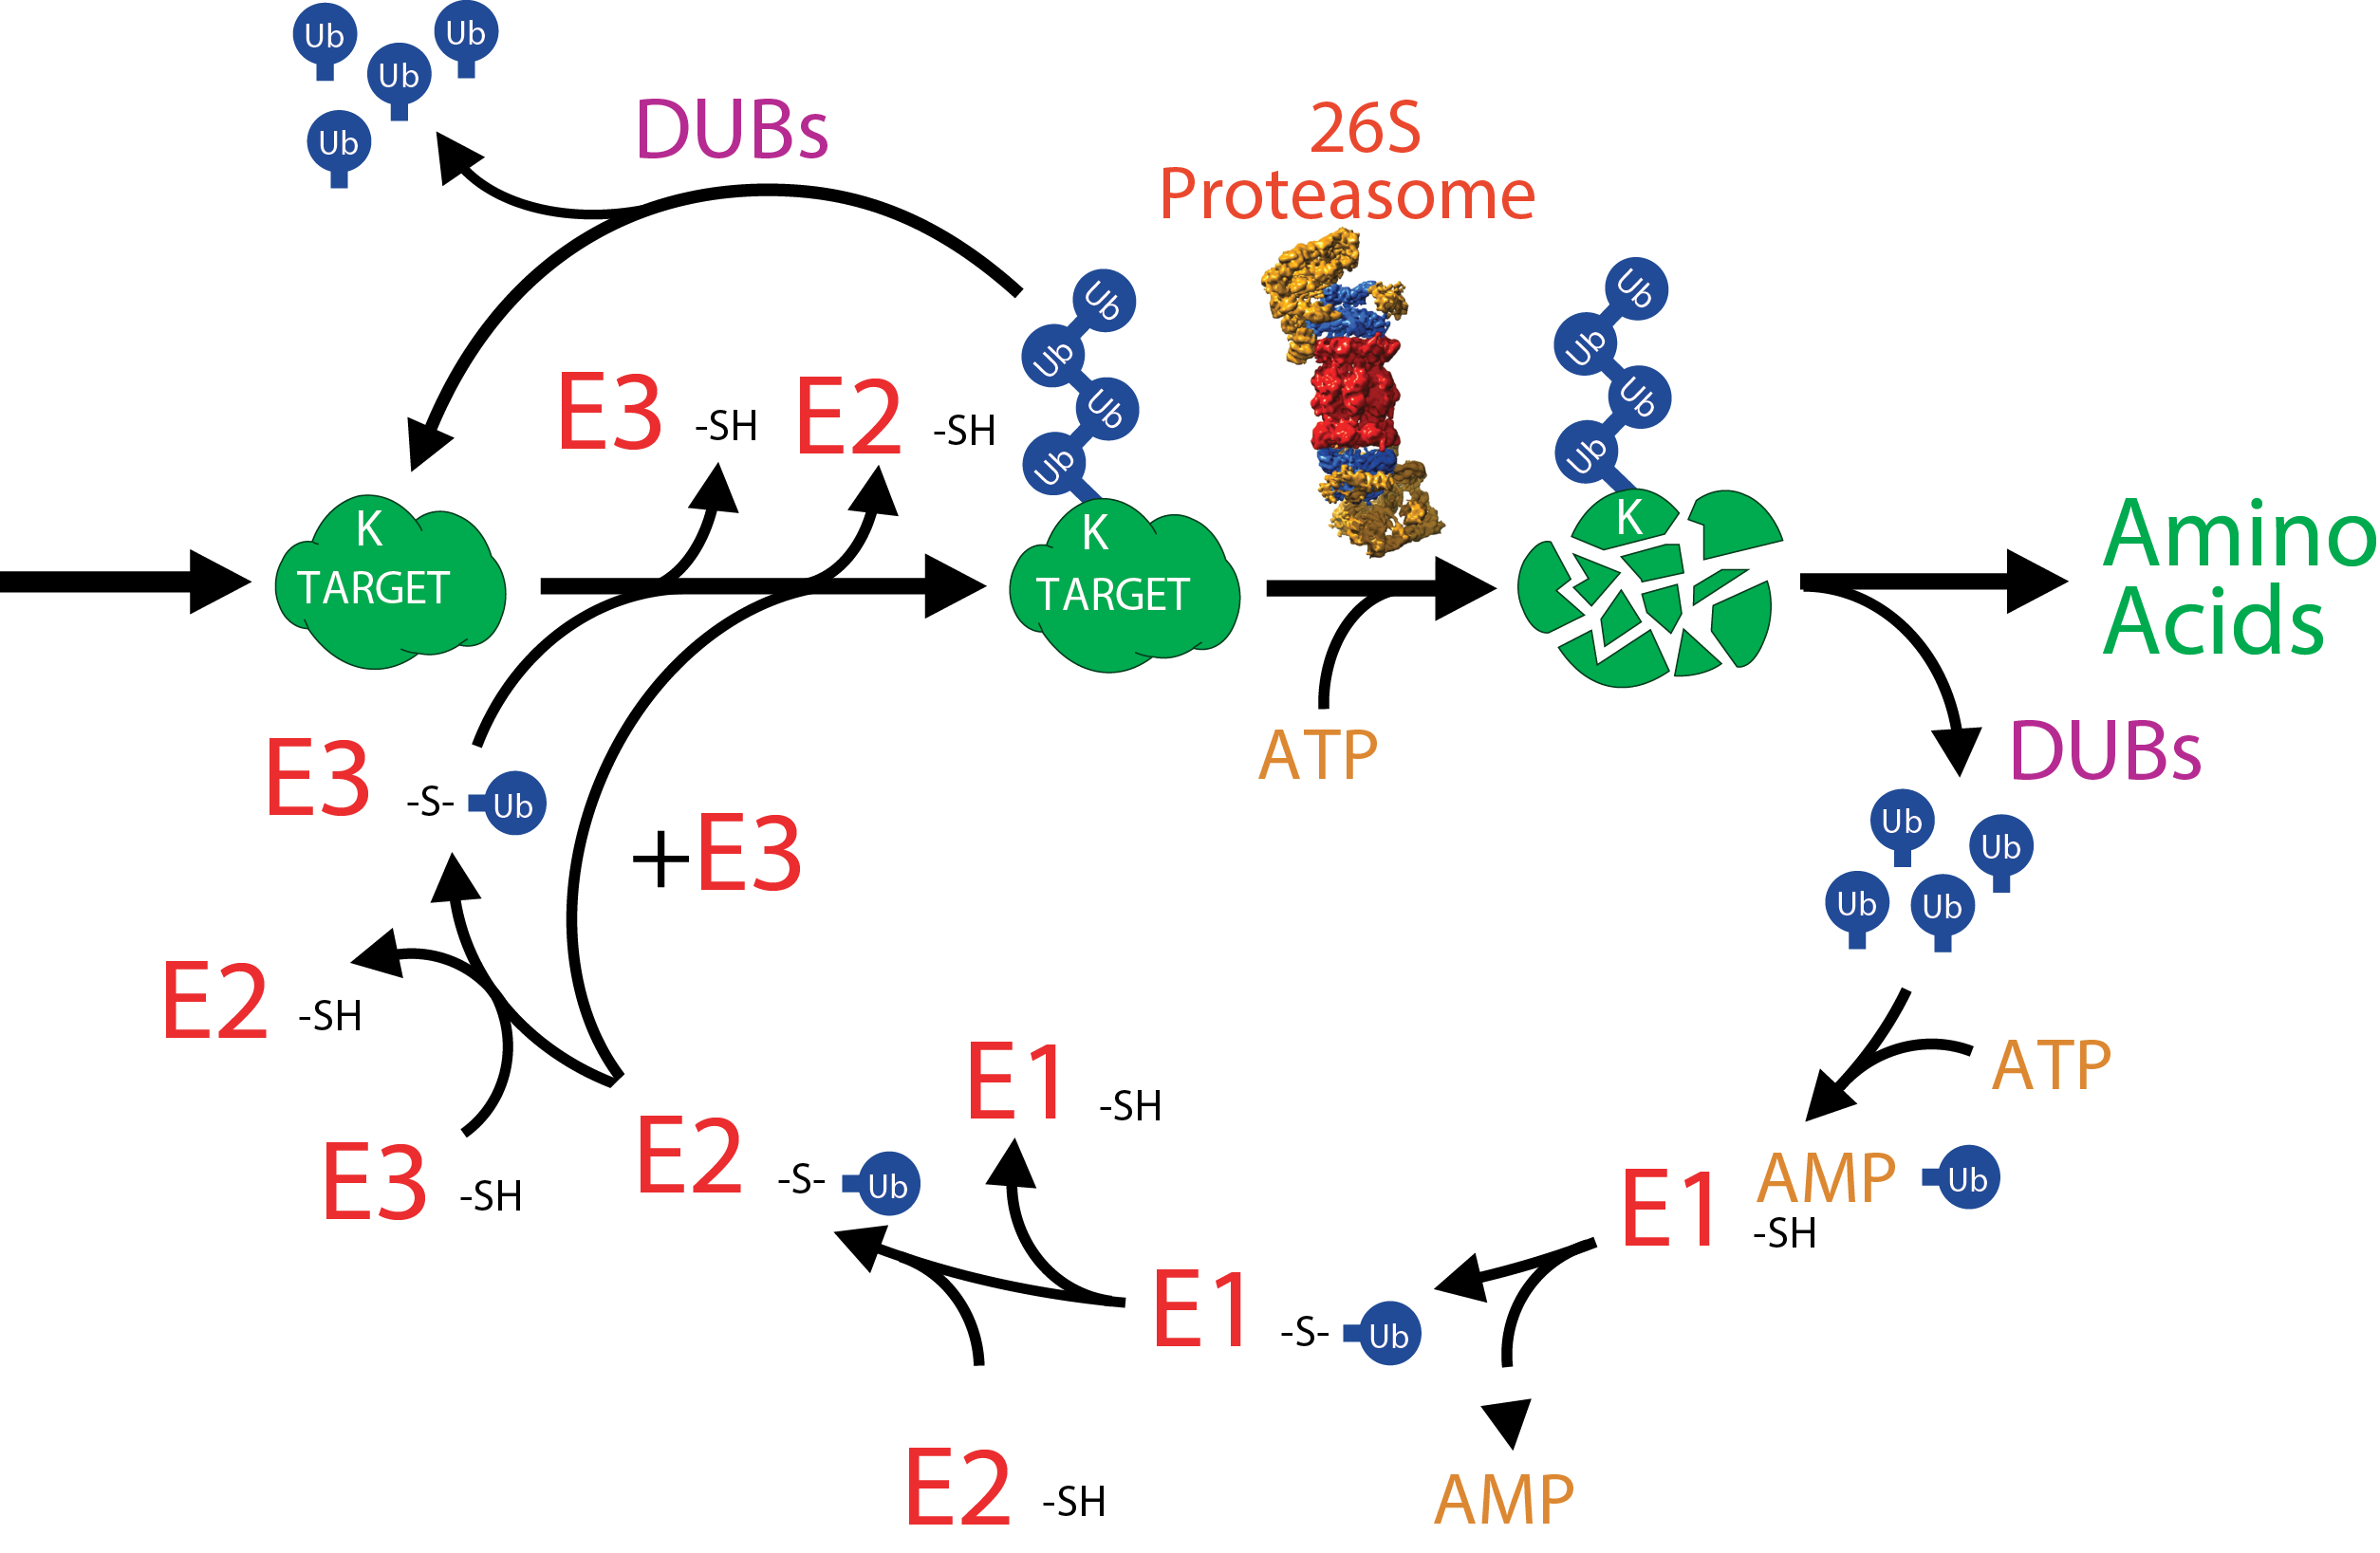
\includegraphics[width=\columnwidth]{intro/upscycle.png}
	\mycaption{The Ubiquitin 26S Proteasome System}{
	Target proteins are covalently modified by ubiquitin an ATP-dependent E1 activating, E2 conjugating, E3 ligase enzymatic cascade. Once a target protein becomes polyubiquitylated, typically with a K48 linkage, it is efficiently recognized and subsequently degraded by the 26S proteasome.  Ubiquitin is released from the target protein by various de-ubiquitylating enzymes (DUBs) and can then enter the cycle again to covalently modify other substrates. 
	}
	\label{fig:UPScycle}
\end{sidewaysfigure}
\section{The 26S Proteasome}
	The 26S proteasome is a 2.5 MDa particle located in the cytosol and nucleus of eukaryotic cells.  It is composed of two functionally distinct sub-complexes; the 20S core protease (CP) that houses the proteolytic active sites, and the 19S regulatory particle (RP) that recognizes appropriate substrates (Figures \ref{fig:proteasomefunc} A and B; \citep{bhattacharyya14, finley09, lander12, lasker12, unverdorben14}).
\begin{figure}[p]
	\centering
	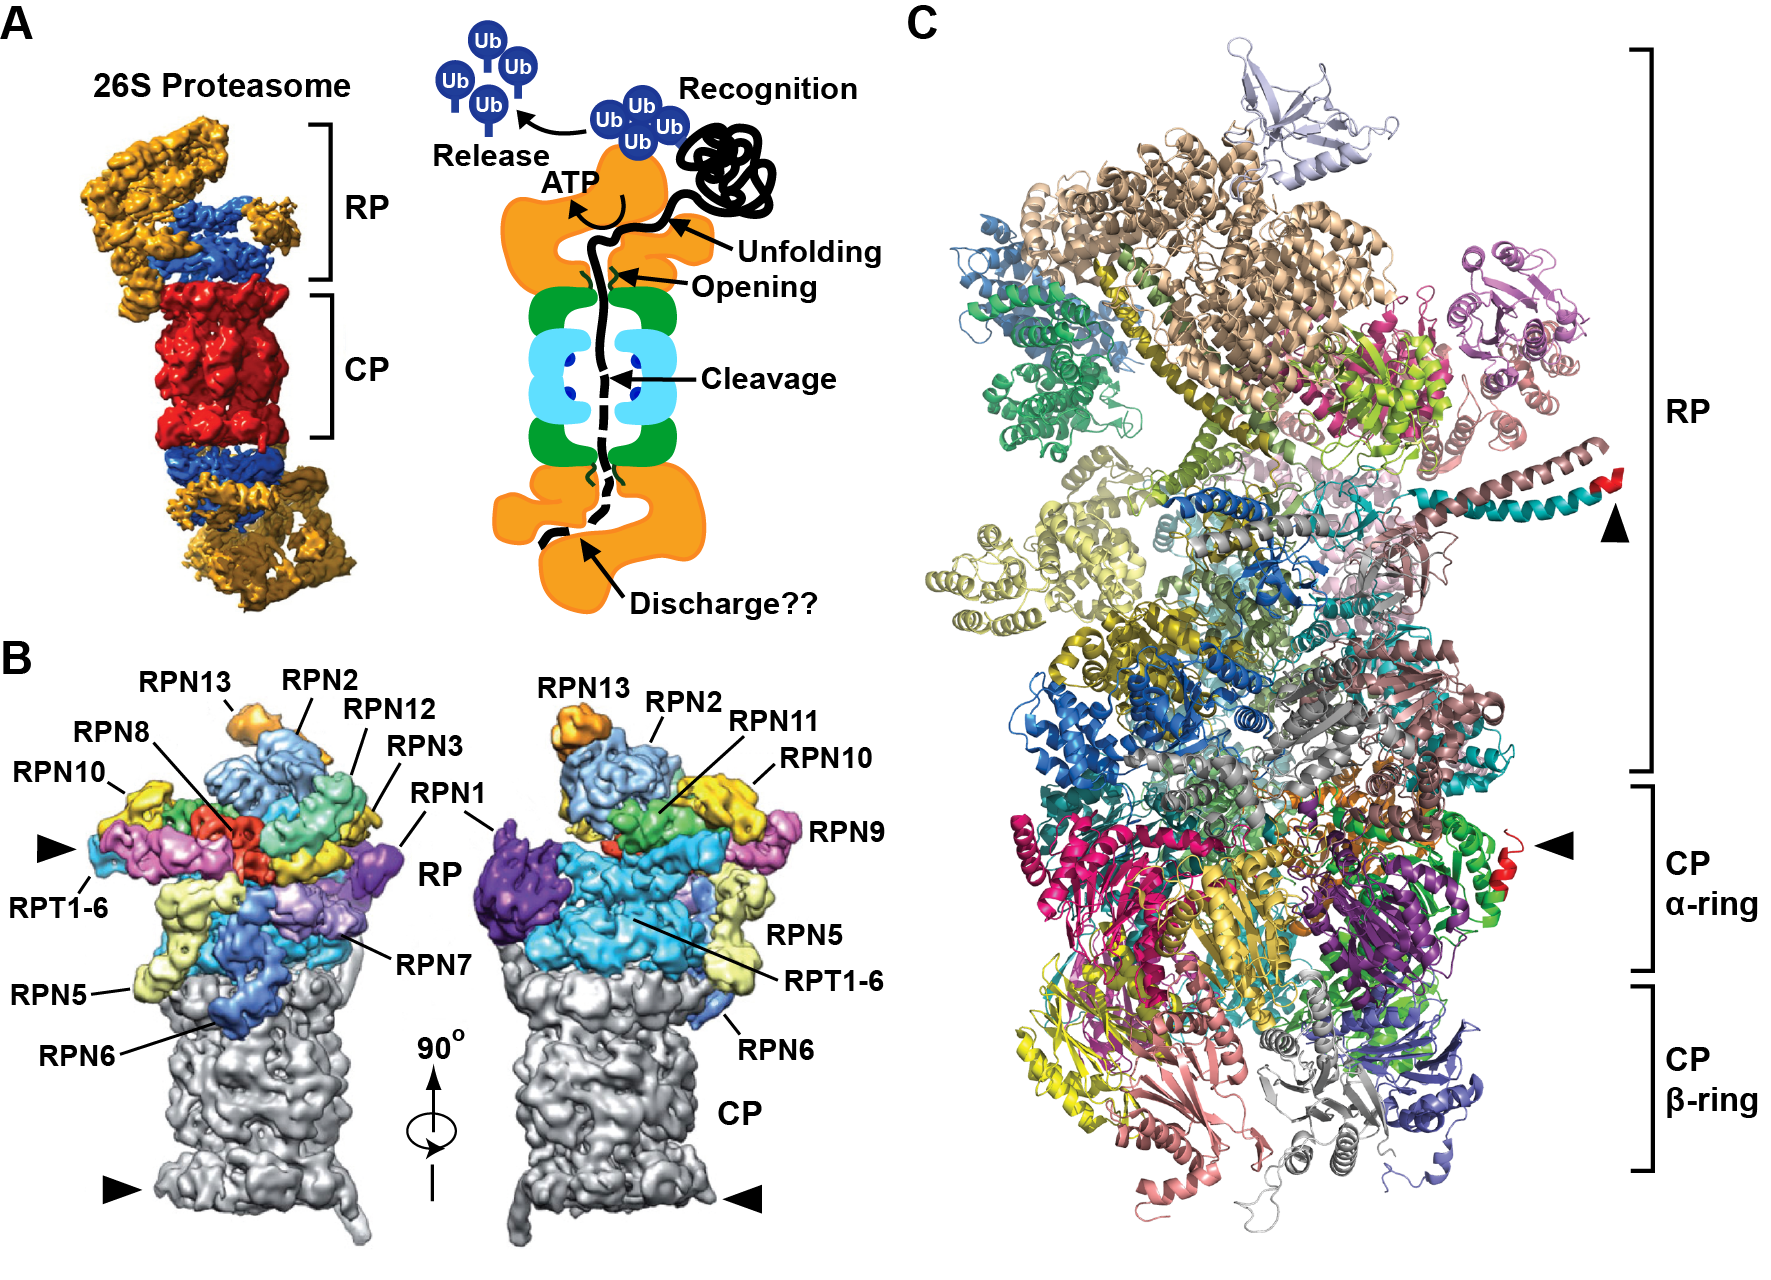
\includegraphics[width=\columnwidth]{intro/figure1.png}
	\mycaption{Structure of the 26S proteasome}{
		\textbf{(A)} Schematic representation of the 26S proteasome, with a 3-D structure as determined by electron microscopy (EM) shown on the left, and a cartoon representation of the holoprotease shown on the right.  Within the EM structure, the CP is shown in red, the RP base is shown in blue, and the RP lid is shown in yellow.  Specific functions within the CP and RP are shown on the right.  The EM structure is modified from reference \citep{lasker12} \textbf{(B)} A detailed view of the subunit architecture of the 26S proteasome RP.  The CP is shown in grey, the RPT ring is shown in blue, and all additional RPN subunits are shown in different colors, with their identity labelled.  The positions of the FLAG tags on PAG1 and RPT4 are indicated by red arrowheads.  These structures are modified from reference \citep{lander12}.  \textbf{(C)} A structural model of the 26S proteasome from yeast at sub-atomic resolution modified from PDB ID 4CR2 \citep{beck12}.  The RP subunits, as well as the CP $\alpha$ and $\beta$ rings are shown.  Highlighted in red, and indicated by black arrowheads, are the positions where FLAG affinity tags have been successfully used to enrich for Arabidopsis 26S proteasomes. The affinity purification of the RP developed as part of the dissertation (Chapter 3) exploits the tag shown in the regulatory particle.
	}
	\label{fig:proteasomefunc}
\end{figure}
	 The CP has a barrel shape generated by four stacked hetero-heptameric rings, which contain seven $\alpha$-subunits or seven $\beta$-subunits (termed PAA-PAG and PBA-PBG, respectively, in \textit{Arabidopsis}) in an $\alpha$1-7/$\beta$1-7/$\beta$1-7/$\alpha$1-7 configuration.  Upon assembly, a central chamber is formed at the $\beta$-ring interface that houses six peptidase catalytic sites provided by the $\beta$1 (PBA), $\beta$2 (PBB), and $\beta$5 (PBE) subunits \citep{arendt97, heinemeyer97}.  The active sites involve a catalytic triad, one residue of which is an N-terminal threonine that becomes exposed during CP assembly.  Collectively these peptidases can cleave a broad range of protein sequences with peptidylglutamyl-peptide hydrolyzing (PGPH) ($\beta$1), trypsin-like ($\beta$2), and chymotryptic-like ($\beta$5) activities  \citep{arendt97, groll99}.  The $\alpha$-rings create two antechambers with narrow opposing axial pores that are gated by extensions at the N-terminus of several subunits \citep{groll00, ruschak10}.  Through this distinctive architecture, the CP acts as a self-compartmentalized protease that will only degrade polypeptides that are deliberately recognized, unfolded, and imported into the $\beta$-ring chamber. 
	The CP is capped at one or both ends by the RP, which sits on top of the axial pores.  The RP provides activities for recognition of ubiquitylated proteins, substrate unfolding and import, and release of the ubiquitin moieties before substrate degradation.  Its binding to the CP is stabilized by ATP, which is thus a necessary ingredient for purifying intact 26S proteasomes.  The RP itself consists of two sub-complexes; the base, which contains a hexameric ring of AAA-ATPases (RPT1-6) plus two non-ATPase subunits, RPN1 and RPN2; and the lid, which is composed of an additional 11 non-ATPase subunits, RPN3, RPN5-13 and DSS1/SEM1 (Figures \ref{fig:proteasomefunc} B and C; \citep{bhattacharyya14, book10, finley09, glickman98-c8Wsa, russell13}.  This lid/base demarcation was first revealed by the absence of lid subunits in proteasomes isolated from a $\Delta$rpn10 yeast deletion strain, and it was hence thought that RPN10 helps enforce binding of the lid to the base \citep{glickman98}.  However, more recent structural studies have demonstrated that RPN10 has a more indirect stabilizing role via its interaction with RPN9 \citep{lander12}.  The ring of RPT subunits in the base promotes substrate unfolding through ATP hydrolysis, and gates the $\alpha$-ring axial pores through repositioning of the CP $\alpha$-subunit extensions \citep{köhler01, rabl08, smith05}.  The N-terminal regions from proximal RPT pairs intertwine to create three spokes onto which most RPN subunits are scaffolded (Figure \ref{fig:proteasomefunc} C; \citep{beck12}).  The RPN6 subunit acts as a molecular clamp to tether the RP onto the CP (Figure \ref{fig:proteasomefunc} B; \citep{pathare12}. 


\section{Proteasome Purification Strategies}
	Even before the realization that the 26S proteasome is a protease, sub-particles of the complexes were described.  The first reports of proteasomes used avian erythroblast preparations enriched by differential ultracentrifugation followed by fractionation through a sucrose gradient \citep{schmid84}.  These 20S fractions isolated in the absence of added ATP were found to inhibit mRNA translation in a cell-free system, leading to early proposals that the identified complex repressed gene expression through a cryptic ribonuclease activity.  This lead to the particle initially being named the ``prosome'' \citep{kremp86, schmid84}.  Subsequent analyses of these preparations by SDS-PAGE and electron microscopy revealed the signature ladder of $\alpha$- and $\beta$-subunits at 20-35 kDa, as well as their barrel-like architecture (Figures \ref{fig:proteasomeelec} A and B; \citep{baumeister88, kremp86, schmid84}).
\begin{figure}[p]
	\centering
	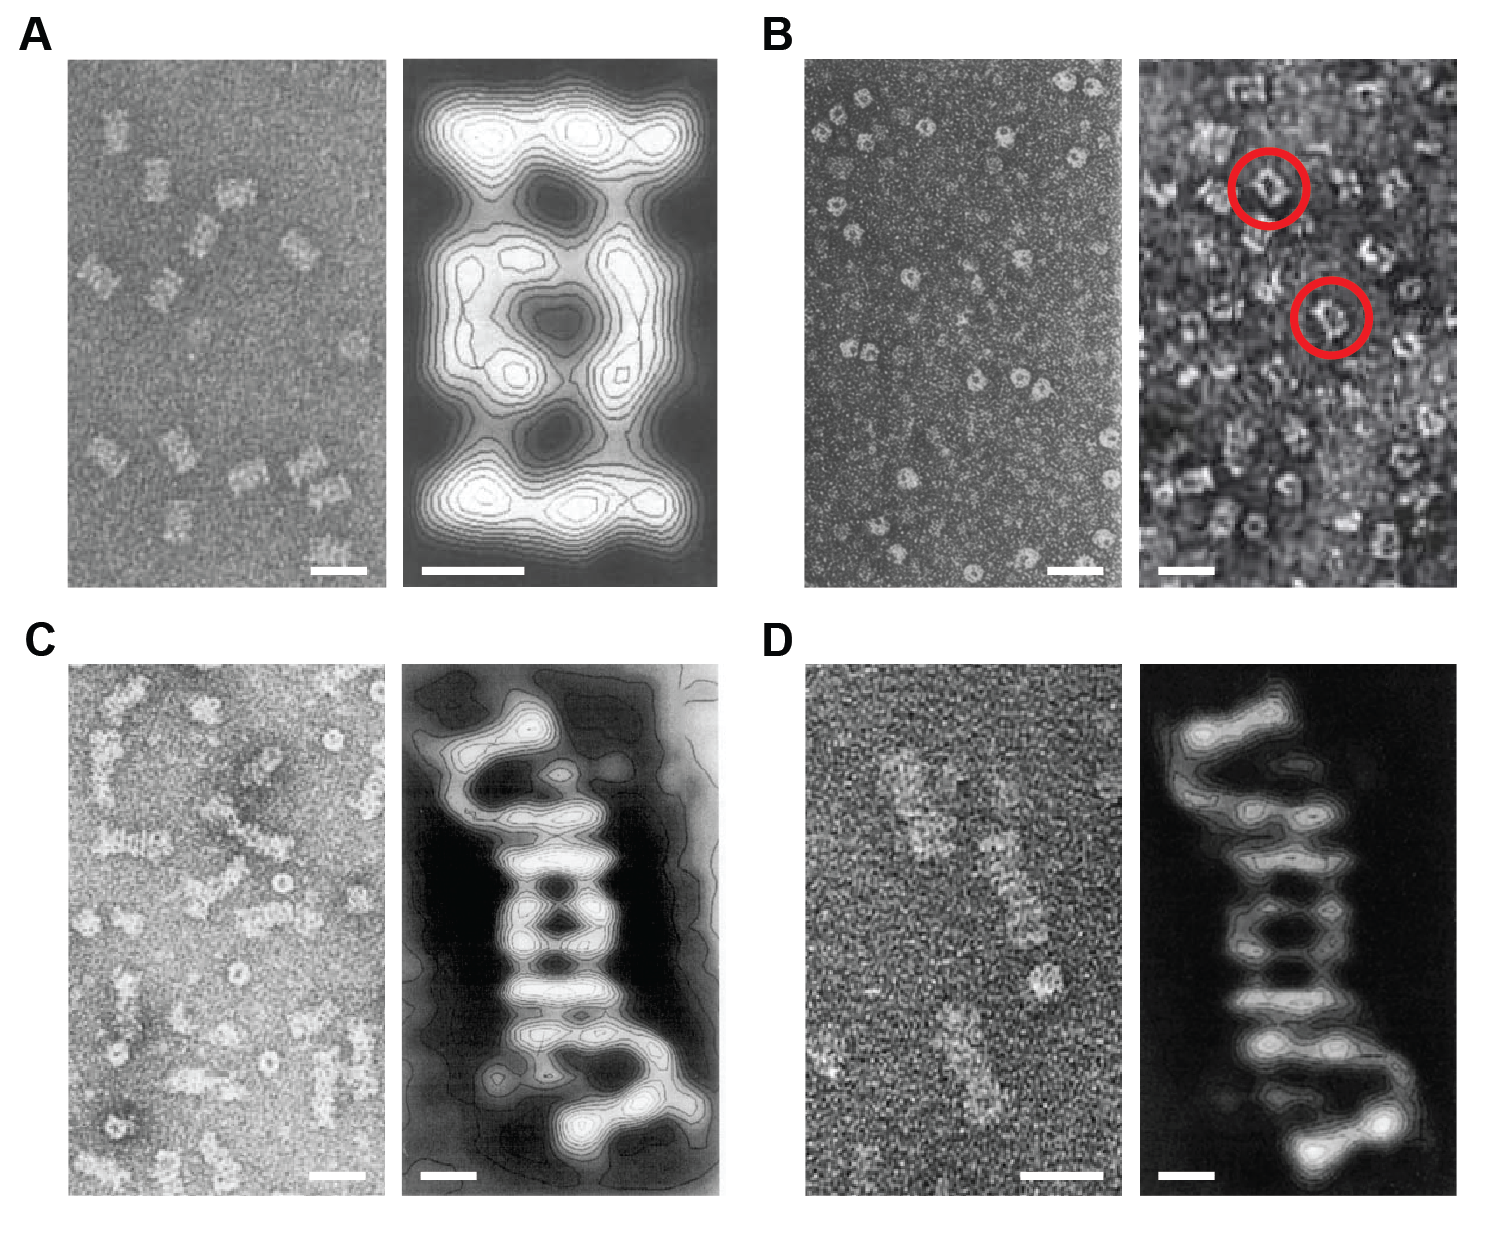
\includegraphics[width=\columnwidth]{intro/figure2.png}
	\mycaption{Electron microscopy images of the 20S and 26S proteasomes from mammals and plants}{
		\textbf{(A)} Images of 20S proteasomes purified from rat skeletal muscle.  On the left is an electron micrograph of the 20S particles negatively stained with sodium phosphotungstate, while on the right is a close-up image with overlaid contour plots generated by correlation averaging of approximately 300 individual images negatively stained with ammonium molybdate.  \textbf{(B)} Images of the first 20S proteasomes purified from different plant species.  On the left are proteasomes isolated from tobacco leaves, while on the right are proteasomes from potato tubers, both negatively stained with uranyl acetate.  The typical barrel-shaped structures are indicated with red circles.  \textbf{(C)} Images of 26S proteasomes purified from rat liver.  On the left is an electron micrograph of the 26S particles negatively stained with uranyl acetate, while on the right is a close-up image with overlaid contour plots generated by correlation averaging of 215 individual images.  \textbf{(D)} Images of 26S proteasomes purified from spinach leaves.  On the left is an electron micrograph of the 26S particles negatively stained with uranyl acetate, while on the right is a close-up image with overlaid contour plots generated by correlation averaging of 450 individual images.  In all cases, scale bars represent 25 nm for the electron micrograph images and 5 nm for close-up images generated by averaging.  The images were modified from references \citep{baumeister88, fujinami94, kremp86, schliephacke91, yoshimura93}.
	}
	\label{fig:proteasomeelec}
\end{figure}
	  Purification of the 20S fraction from HeLa cells followed by SDS-PAGE also gave rise to this stereotypical protein banding pattern and shape \citep{schmid84}, and this was followed shortly thereafter by the first description of plant prosomes, purified from tobacco leaf extracts using similar sedimentation protocols in ATP-free buffers \citep{kremp86}.  In these later cases, the purified preparations had strong peptidase activity but little to no RNase activity, thus leading to the conclusion that the CP is actually a protease.  Once its true function in protein turnover was confirmed, the moniker for the particle was changed to `proteasome' \citep{arrigo88}.  
	Subsequently, the 20S particle was purified from other plant tissues, including dry pea seeds, potato tubers, mung bean seedlings, and leaves from both spinach and wheat \citep{murray97, ozaki92, schliephacke91, skoda92}.  These purifications were typically performed using sequential anion exchange and size-exclusion chromatography steps in the absence of ATP, hence only the CP was isolated.  Their remarkable similarity in protein composition and structure, as observed by SDS-PAGE and electron microscopy, respectively, coupled with the fact that several of the plant subunits cross-reacted with antibodies against their yeast, human, rat and Xenopus counterparts, strongly implied that the CP was conserved and widely distributed among eukaryotes \citep{schliephacke91}.
	The complete 26S proteasome (i.e. the CP capped at one or both ends by the RP) was subsequently discovered by the purification of ubiquitin conjugate-degrading activity from rabbit reticulocytes \citep{hough86}.  While it had been well established that major catabolic processes in animal cells involved the ATP-dependent proteolysis of selective substrates \citep{etlinger77}, the enzyme(s) responsible for this activity had yet to be identified.  Taking advantage of the new ability to synthesize ubiquitylated substrates such as 125I-labelled ubiquitin-lysozyme conjugates \citep{hough86-1xVPf}, a protocol was developed to purify the responsible ATP-dependent protease.  Through a series of anion exchange and size exclusion chromatography steps followed by glycerol gradient sedimentation, all of which were performed in ATP-containing buffers, the responsible activity was isolated \citep{hough86, hough87}. The active enzyme turned out to be the 20S proteasome (i.e. the CP) along with a number of additional polypeptides which together formed a 26S particle, thus providing the first direct link between ubiquitylation and a protease \citep{ganoth88, hough87, waxman87}.  SDS-PAGE analysis of these preparations identified a host of new polypeptides in the 35-100 kDa range in addition to the known CP subunits, which were later shown to comprise a second stable complex, the RP.  Shortly thereafter, the RP was demonstrated to have ATPase activities attributable to the RPT subunits, which help in substrate unfolding and maintaining CP-RP association \citep{armon90}.  Electron microscopic images of the full 26S particle then revealed its diagnostic quaternary structure in which the CP is capped by one or two RPs which sit over the axial pores for substrate entry (Figure \ref{fig:proteasomeelec} C; \citep{peters91, yoshimura93}).
	The existence of a similar 26S proteasome in plants was initially implied by the detection of an ATP-dependent activity in oat and wheat germ extracts capable of degrading ubiquitylated proteins \citep{hatfield89, vierstra88}.  This was followed some years later by the first isolation of a complete plant 26S proteasome holocomplex from spinach leaves \citep{fujinami94}.  As with the mammalian forms, purification was achieved by anion exchange and size exclusion chromatography, followed by glycerol gradient centrifugation, all in the presence of ATP to stabilize the CP-RP association.  These spinach preparations were, like their rabbit reticulocyte counterparts, able to rapidly degrade ubiquitylated substrates in an ATP-dependent manner, and further analysis by native-PAGE, SDS-PAGE and electron microscopy revealed the complete subunit composition and ``caterpillar-like'' structure of the plant particle (Figure \ref{fig:proteasomeelec} D; \citep{fujinami94}).  Similar purifications were successful using rice suspension culture cells and garlic cloves \citep{malik04, yanagawa99}, which were accompanied by the first demonstrations that proteasome inhibitors designed for their mammalian counterparts were effective with the plant particles, suggesting very similar enzymatic mechanisms \citep{ozaki92, woffenden98}.
	Despite its prevalence as a genetic model, purification of the 26S proteasome from the flowering plant \textit{Arabidopsis thaliana} was not reported until several years after other plant species \citep{yang04}.  First protocols involved differential PEG precipitation followed by anion exchange and size exclusion chromatography, with the latter exploiting the large size of the holoprotease.  More recently, an improved one-step affinity method was developed \citep{book10}, based on the strategies that had been successfully employed in yeast \citep{leggett05}.  Here, epitope-tagged proteasomes were generated by genetically replacing the subunit PAG1 with a variant bearing a C-terminal FLAG tag; this tagged particle could then be purified with appropriate affinity matrices and released in its native condition with FLAG peptide.  This approach enables rapid and robust purification of the whole 26S proteasome complex when performed in the presence of ATP, or enables purification of the CP sub-particle when performed in the absence of ATP \citep{book10}. This affinity method has considerable advantages compared to previous conventional chromatographic approaches \citep{yang04} as it is both faster and more reliable, produces higher yields per gram of tissue (~6 µg/g)..
\begin{figure}[p]
	\centering
	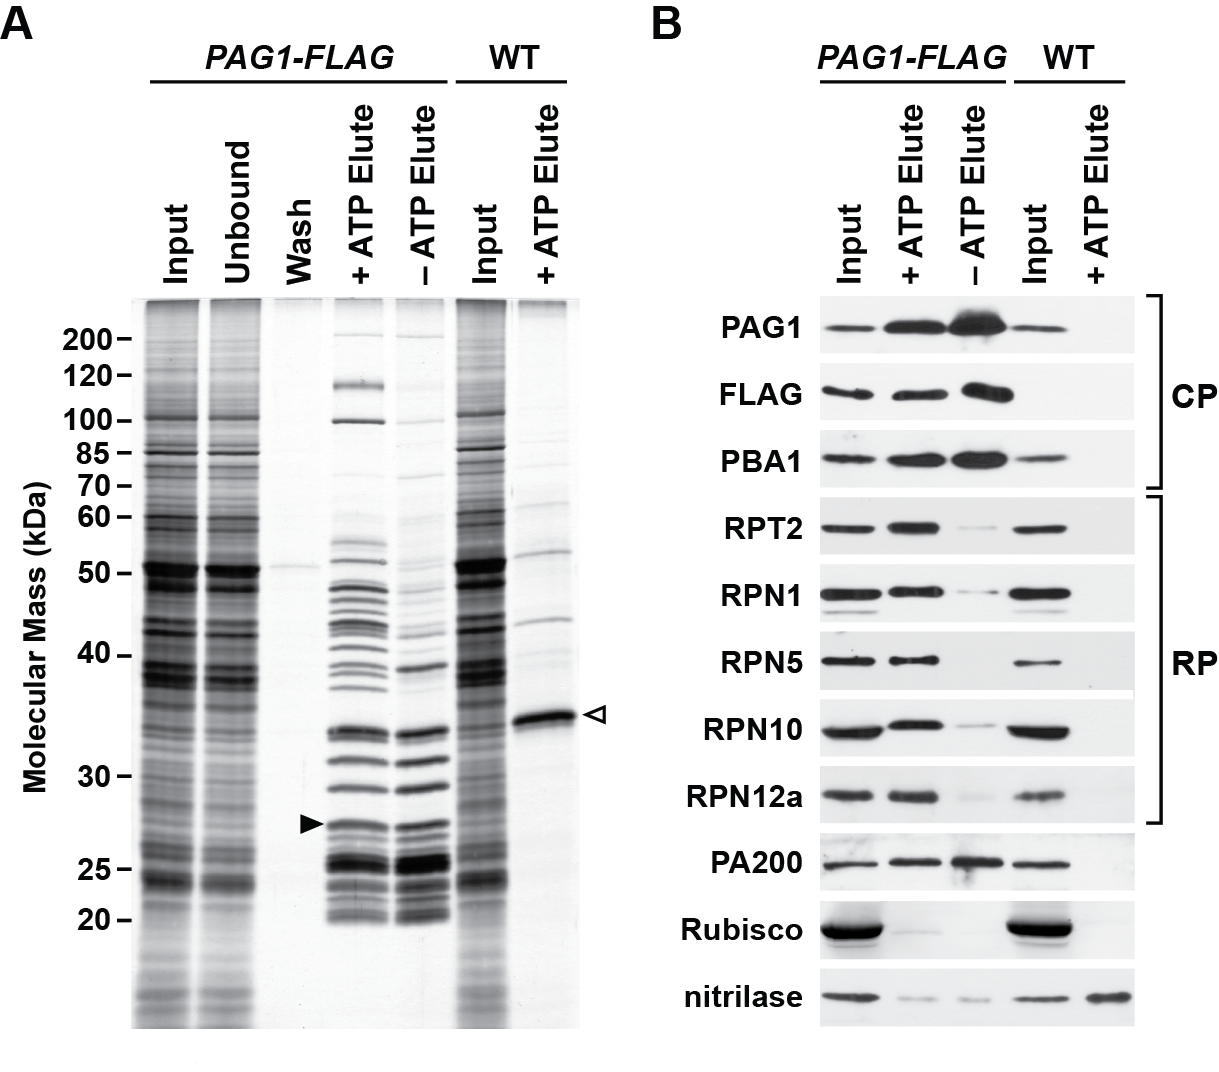
\includegraphics[width=\columnwidth]{intro/pag1affinity.png}
	\mycaption{Affinity purification of 26S proteasomes from \textit{pag1-1 PAG1-FLAG} plants}{
		\textbf{(A)} SDS-PAGE analysis of the affinity purification steps.  Total protein extracts from 10 day old wild-type (WT) and \textit{pag1-1 PAG1-FLAG} plants were incubated with anti-FLAG affinity resin, washed, and competitively eluted with the FLAG peptide.  The procedure was performed in the presence or absence of ATP, and the input, unbound, washed and eluted fractions were subjected to SDS-PAGE and the gel stained for protein with silver.  The black arrowhead indicates the PAG1-FLAG protein, while the open arrowhead identifies nitrilase, which is non-specifically enriched during the purification.  \textbf{(B)} Immunoblot detection of various 26S proteasome subunits in the affinity-purified preparations shown in A. Subunits tested include the CP subunits PAG1 and PBA1, the RP subunits RPT2, RPN1, RPN5, RPN10 and RPN12a, and the alternate capping particle PA200.  Other proteins tested include the Rubisco small subunit and nitrilase.  This figure was modified from reference \citep{book10}.
	}
	\label{fig:pag1affinity}
\end{figure}
This milder more rapid technique also prevents breakdown of some subunits, in particular RPN10, which is sensitive to post-homogenization proteolysis \citep{yang04}.  One caveat is that the epitope tag, given its exposed position and flexible structure, might be sensitive to proteolytic cleavage following tissue homogenization.  For the PAG1-FLAG protocol, chymostatin was found to effectively block the interfering protease \citep{book10}.  An example of such preparations analyzed by SDS-PAGE followed by immunoblotting with antibodies against several proteasome subunits, are shown in Figures  \ref{fig:pag1affinity} A and B, respectively.


\section{26S Proteasome Substrate Processing}
	A variety of proteins help the 26S proteasome process ubiquitylated substrates. Some include key constituents of the complex itself such as RPN11, which is a metalloprotease that uses a zinc-coordinated active site to release the ubiquitin moieties isopeptide-linked to substrates \citep{verma02, worden14}.  Through RPN11 and other loosely associated deubiquitylating enzymes such as UBP6/USP14 \citep{hanna06, sakata11}, bound ubiquitins are actively recycled.
	Substrate selection by the 26S proteasome is dictated by several ubiquitin receptors intrinsic to the RP lid, including RPN10, RPN13 (in yeast), and DSS1/SEM1 \citep{fatimababy10, finley09, lin11, paraskevopoulos14, sakata12, van96}, and possibly RPN1 in the base \citep{elsasser02}.  RPN10 binds ubiquitin via defined ubiquitin-interacting motifs (UIMs), of which yeast, human and \textit{Arabidopsis} RPN10 contain 1, 2 and 3 in tandem, respectively \citep{fatimababy10, finley09, fu98, lin11, van96}.  By contrast, RPN13 binds ubiquitin via a pleckstrin-like receptor for ubiquitin (PRU) domain, which is structurally distinct from UIMs but binds to the same hydrophobic patch on ubiquitin \citep{husnjak08, schreiner08}.  More recently, DSS1/SEM1 was also found to be a proteasomal ubiquitin receptor \citep{paraskevopoulos14}.  It had previously resisted identification due to both its small size, which prevented visualization by standard protein stains following sodium dodecyl sulfate-polyacrylamide gel electrophoresis (SDS-PAGE), and its paucity of lysine and arginine residues, which complicated detection by conventional mass spectrometric methods.  Only with the use of top-down mass spectrometry of 26S proteasome complexes was DSS1/SEM1 first detected in intact 26S proteasomes from \textit{Arabidopsis} \citep{russell13}.  
	In addition to these core ubiquitin receptors, there are several extra-proteasomal ubiquitin-binding proteins that shuttle ubiquitylated cargo to the RP.  They work by virtue of ubiquitin-associated (UBA) domains that bind ubiquitin, combined with a ubiquitin-like (UBL) domain that interacts with the intrinsic ubiquitin receptors such as RPN10.  Important shuttle factors in plants include RAD23, DSK2, and DDI1 \citep{farmer10, fatimababy10, finley09, lin11}, though many other ubiquitin-binding proteins are known in other species \citep{husnjak12}.  Numerous other factors also associate sub-stoichiometrically with the mature CP and RP sub-complexes, including deubiquitylating enzymes, several E3 ligases and protein kinases, and a collection of protein folding chaperones \citep{besche14, book10, leggett02, xie00}.


\section{Proteasome Isotypes}
	Genetic Analysis of CP and RP subunits shows lethality etc


\section{Proteasome Inhibition and Proteasome Degredation}


\section{26S Proteasome Assembly}
	Not surprisingly given its intricate architecture, construction of the 26S proteasome requires a large collection of assembly factors that work in synchrony.  Included are chaperones required for the correctly ordered assembly of the $\alpha$- and $\beta$-rings of the CP and the RPT ring of the RP, which in yeast involve the Pba1/2 and Pba3/4 heterodimers for the CP \citep{kusmierczyk08, le07, tomko13}, and Nas2, Nas6, Hsm3 and Rpn14 for the RP \citep{funakoshi09, roelofs09, saeki09, tomko13}.  Additional chaperones then mediate assembly of the final particle.  UMP1 is required to connect the two $\alpha$/$\beta$ half-barrels to generate the complete CP.  Once its job is finished UMP1 is degraded, thus becoming the first proteolytic substrate of the fully assembled CP \citep{ramos98}.  ECM29 stabilizes the association of assembled CP and RP and provides a final quality control checkpoint for mature 26S proteasomes \citep{besche14, lehmann10}.  Finally, in some situations, the RP is replaced entirely by alternate capping particles such as PA200 (also known as Blm10) or CDC48 \citep{barthelme12, book10, schmidt05}.  The functions of these caps are not yet clear, but recent proposals for PA200 have it participating in 26S proteasome assembly, helping shuttle proteasomes into the nucleus, and/or generating a ubiquitin-independent proteasome containing CP and PA200 only \citep{dange11, sadre-bazzaz10, weberruss13}.


\section{Proteasome Associated Proteins (PAPs)}
Beyond those associated proteins already mentioned that are involved in substrate processing and assembly, there are a variety of proteins that are known to interact with the yeast and mammalian proteasomes. These include: loosely associated DUBS such as UCH37, and etc etc


\section{Conclusions}

The \textit{Arabidopsis} 26S proteasome exists in planta as a diverse array of complexes containing multiple subunit isoforms and interacting proteins \citep{book10, fu99, yang04}.  To facilitate biochemical analysis of the plant particle, we developed a rapid and robust affinity purification protocol that enables isolation of intact 26S proteasomes, and the individual CP and RP (Chapter 3) sub-complexes, by genetically replacing individual subunits with FLAG-tagged versions \citep{book10}.  Such a strategy was based on a similar approach used successfully with yeast, where the proteasome subunits Pre1, Rpt1 and Rpn11 were appended with either FLAG or Protein A tags to permit effective affinity enrichment \citep{leggett05}.  Using the recently described structures of the 26S proteasome \citep{bhattacharyya14, lander12, lasker12}, we identified subunits in the CP (PAG1) and as demonstrated in this thesis RP (RPT4) which had solvent exposed N- or C-termini that were potentially appropriate for appending the epitope tag (see Figures \ref{fig:proteasomefunc} B and C).  


\begin{singlespace}
\bibliographystyle{plant_cell_final}
\renewcommand\bibname{Literature Cited}
\bibliography{UPS}
\end{singlespace}



\chapter{Morpheus Spectral Counter: A Computational Tool for Label-Free Quantitative Mass Spectrometry using the Morpheus Search Engine}

\section{Summary}
Label-free quantitative MS based on the Normalized Spectral Abundance Factor (NSAF) has emerged as a straightforward and robust method to determine the relative abundance of individual proteins within complex mixtures.
Here, we present Morpheus Spectral Counter (MSpC) as the first computational tool that directly calculates NSAF values from output obtained from Morpheus, a fast, open-source, peptide-MS/MS matching engine compatible with high-resolution accurate-mass instruments.
NSAF has distinct advantages over other MS-based quantification methods, including a higher dynamic range as compared to isobaric tags, no requirement to align and re-extract MS1 peaks, and increased speed.
MSpC features an easy to use graphic user interface that additionally calculates both distributed and unique NSAF values to permit analyses of both protein families and isoforms/proteoforms.
MSpC determinations of protein concentration were linear over several orders of magnitude based on the analysis of several high-mass accuracy datasets either obtained from PRIDE or generated with total cell extracts spiked with purified \textit{Arabidopsis} 20S proteasomes.
The MSpC software was developed in C\# and is open sourced under a permissive license with the code made available at \url{http://dcgemperline.github.io/Morpheus_SpC/}. 

\section{Main Text}
Quantification of individual polypeptides within complex mixtures by MS is an extremely useful tool to understand proteomic changes in organisms during growth and development, and after environmental perturbation \citep{wong10}.
While a number of MS/MS strategies have been developed to measure protein abundance, including Stable Isotope Labeling by Amino Acids in Cell Culture (SILAC), labeling with isobaric tags, and Absolute Quantification of proteins (AQUA) \citep{gerber03, ong02, ross04, thompson03}, label-free quantification (LFQ) have become increasingly popular given their simplicity and low cost \citep{wong10, zhang06}.
One LFQ strategy infers abundance from the number of observed peptide spectra matches (PSMs).
For these PSM-based approaches, changes in protein abundance can be generated artifactually when total PSMs differ among samples and because longer proteins tend to produce more raw counts.
For these reasons normalizing for both protein length and total PSMs is paramount.
While this adjustment can be made in a number of ways; one of the most straight forward methods is to use Normalized Spectral Abundance Factor (NSAF), a length- and count-normalized measure for each protein \citep{zybailov06}.
Further improvements to the NSAF algorithm have been made by accounting for shared peptides in distributed NSAF (dNSAF), which distributes common PSMs among a family of isoforms/proteoforms based on the number of distinct PSMs observed for each isoform/proteoform, and unique NSAF (uNSAF), which ignores shared PSMs and only assigns distinct PSMs to each specific isoform/proteoform \citep{zhang10}.

The Morpheus MS search engine was recently designed for high-resolution, accurate-mass data obtained from Orbitrap-based instruments to provide faster matching of spectra to peptides \citep{wenger13}.
Unfortunately, no downstream automated tools are available to facilitate LFQ analysis, which can be quite challenging, if not impossible, to complete manually when accounting for shared peptides.
To overcome this bottleneck, we developed Morpheus Spectral Counter (MSpC) as the first LFQ computational tool that integrates directly with Morpheus to calculate NSAF, dNSAF, uNSAF, and corrected PSM \citep{fermin11} values in complex protein samples.
\begin{sidewaysfigure}[p]
	\centering
	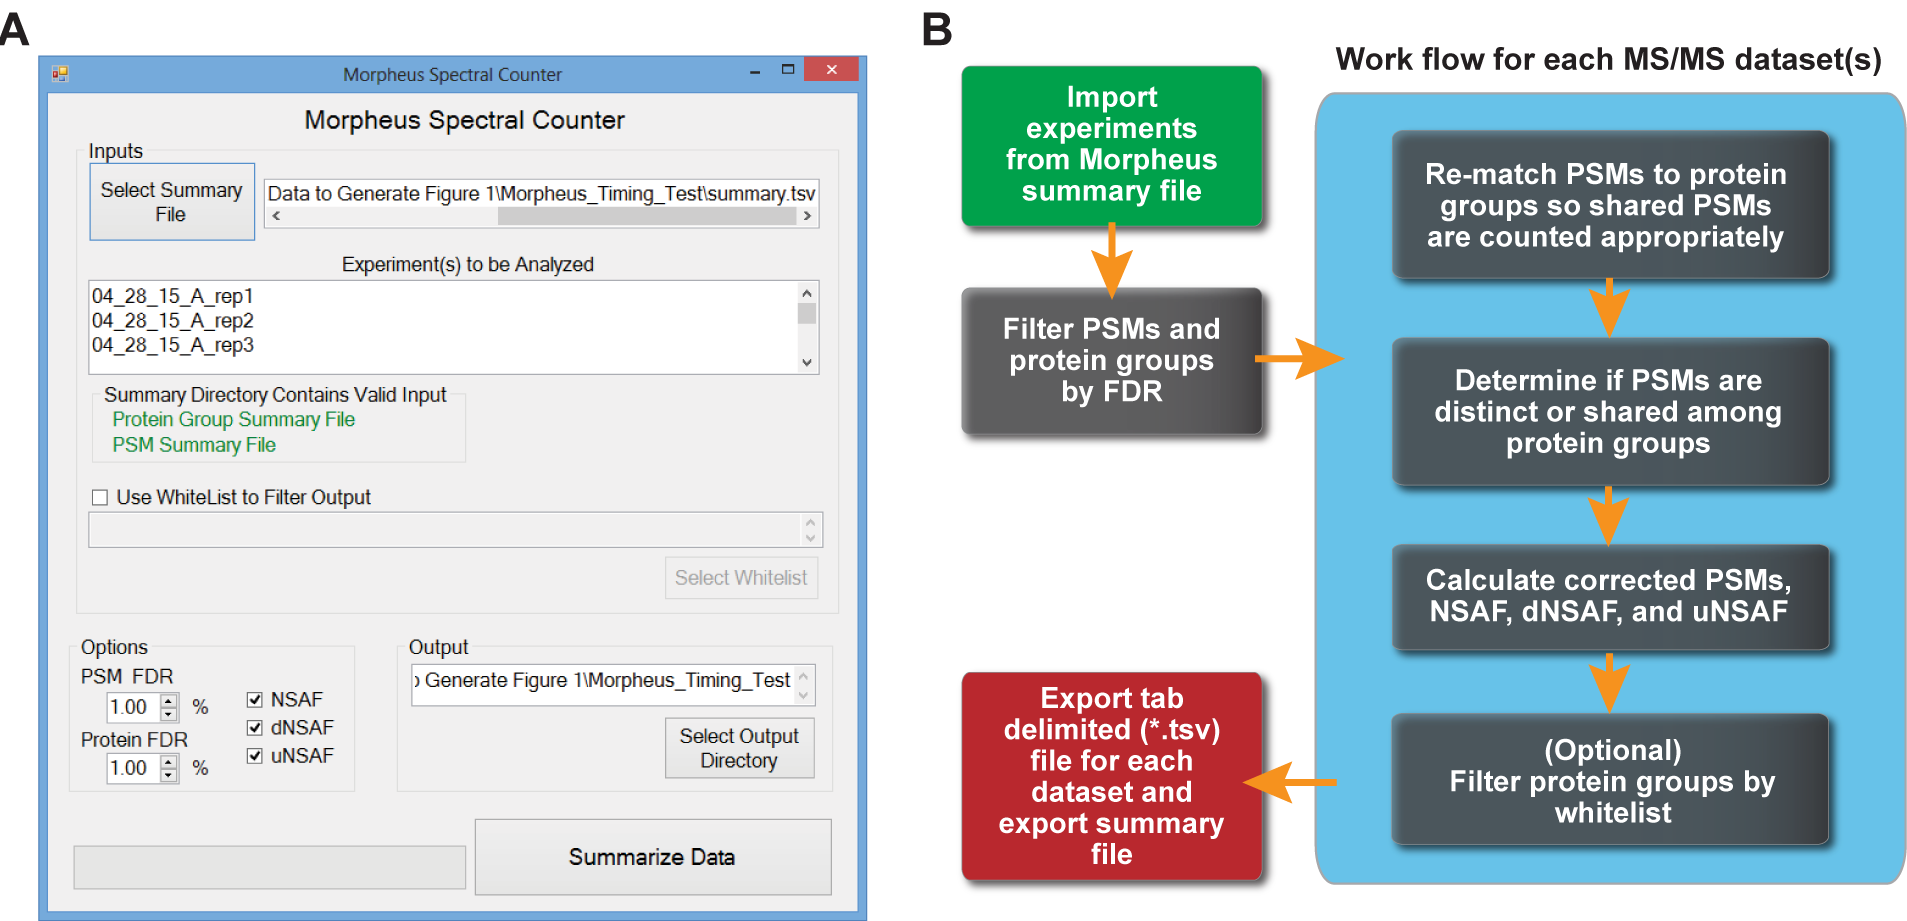
\includegraphics[width=\columnwidth]{MSpC/figure1_supplemental.png}
	\mycaption{MSpC Graphic User Interface (GUI) and software flow chart}{
\textbf(A) Screenshot of the GUI.
The input requires the user to select a Morpheus search summary file containing experiments to be analyzed.  The user can optionally select a whitelist to filter output, and select an output directory.
Additional options can set peptide and protein FDR cutoffs, and method of quantification for output, including Normalized Spectral Abundance Factor (NSAF), distributed NSAF (dNSAF), and unique	NSAF (uNSAF).
A progress bar highlights completion of the analysis.
\textbf(B) Data analysis flow chart.
Experiments and groups of experiments to be analyzed are imported through the Morpheus summary file.
PSMs and protein groups are filtered at the specified FDR cutoff with a default of 1\%.}
	\label{fig:GUIflow}
\end{sidewaysfigure}
MSpC is fully automated, and only requires a Morpheus search summary file (summary.tsv) as input.
The user interface (see Figure \ref{fig:GUIflow} (A)) allows one to select the summary file and displays the raw MS/MS files that will be analyzed by MSpC.
Due to shared peptides being attributed to only one instance of a protein group in Morpheus's PSM file, PSMs are re-matched to all possible protein groups.
PSMs are then cataloged as shared or as unique (distinctly matching one protein group) to generate NSAF, dNSAF, and uNSAF outputs.
Finally, the output can be filtered for proteins of interest by specifying a comma delimited file containing unique identifiers and descriptions.
Some important features of MSpC are its ability to handle fractionation experiments as input, and the ability to whitelist proteins of interest in the output by specifying a csv file (see Tutorial \ref{sec:tutorial}).
Options exist to specify global PSM and protein group FDR rates (thus avoiding increased FDRs when one analyzes many experiments at once), to output NSAF, dNSAF, and uNSAF values, to require a minimum number of unique peptides to quantify a protein, and to specify an output directory.
A progress bar indicates completion of the analysis by MSpC.
To validate the accuracy of MSpC, we analyzed two MS/MS datasets available in PRIDE that were previously generated by high-energy collision-induced dissociation using Thermo Q-Exactive Orbitrap instruments.
\begin{figure}[p]
	\centering
	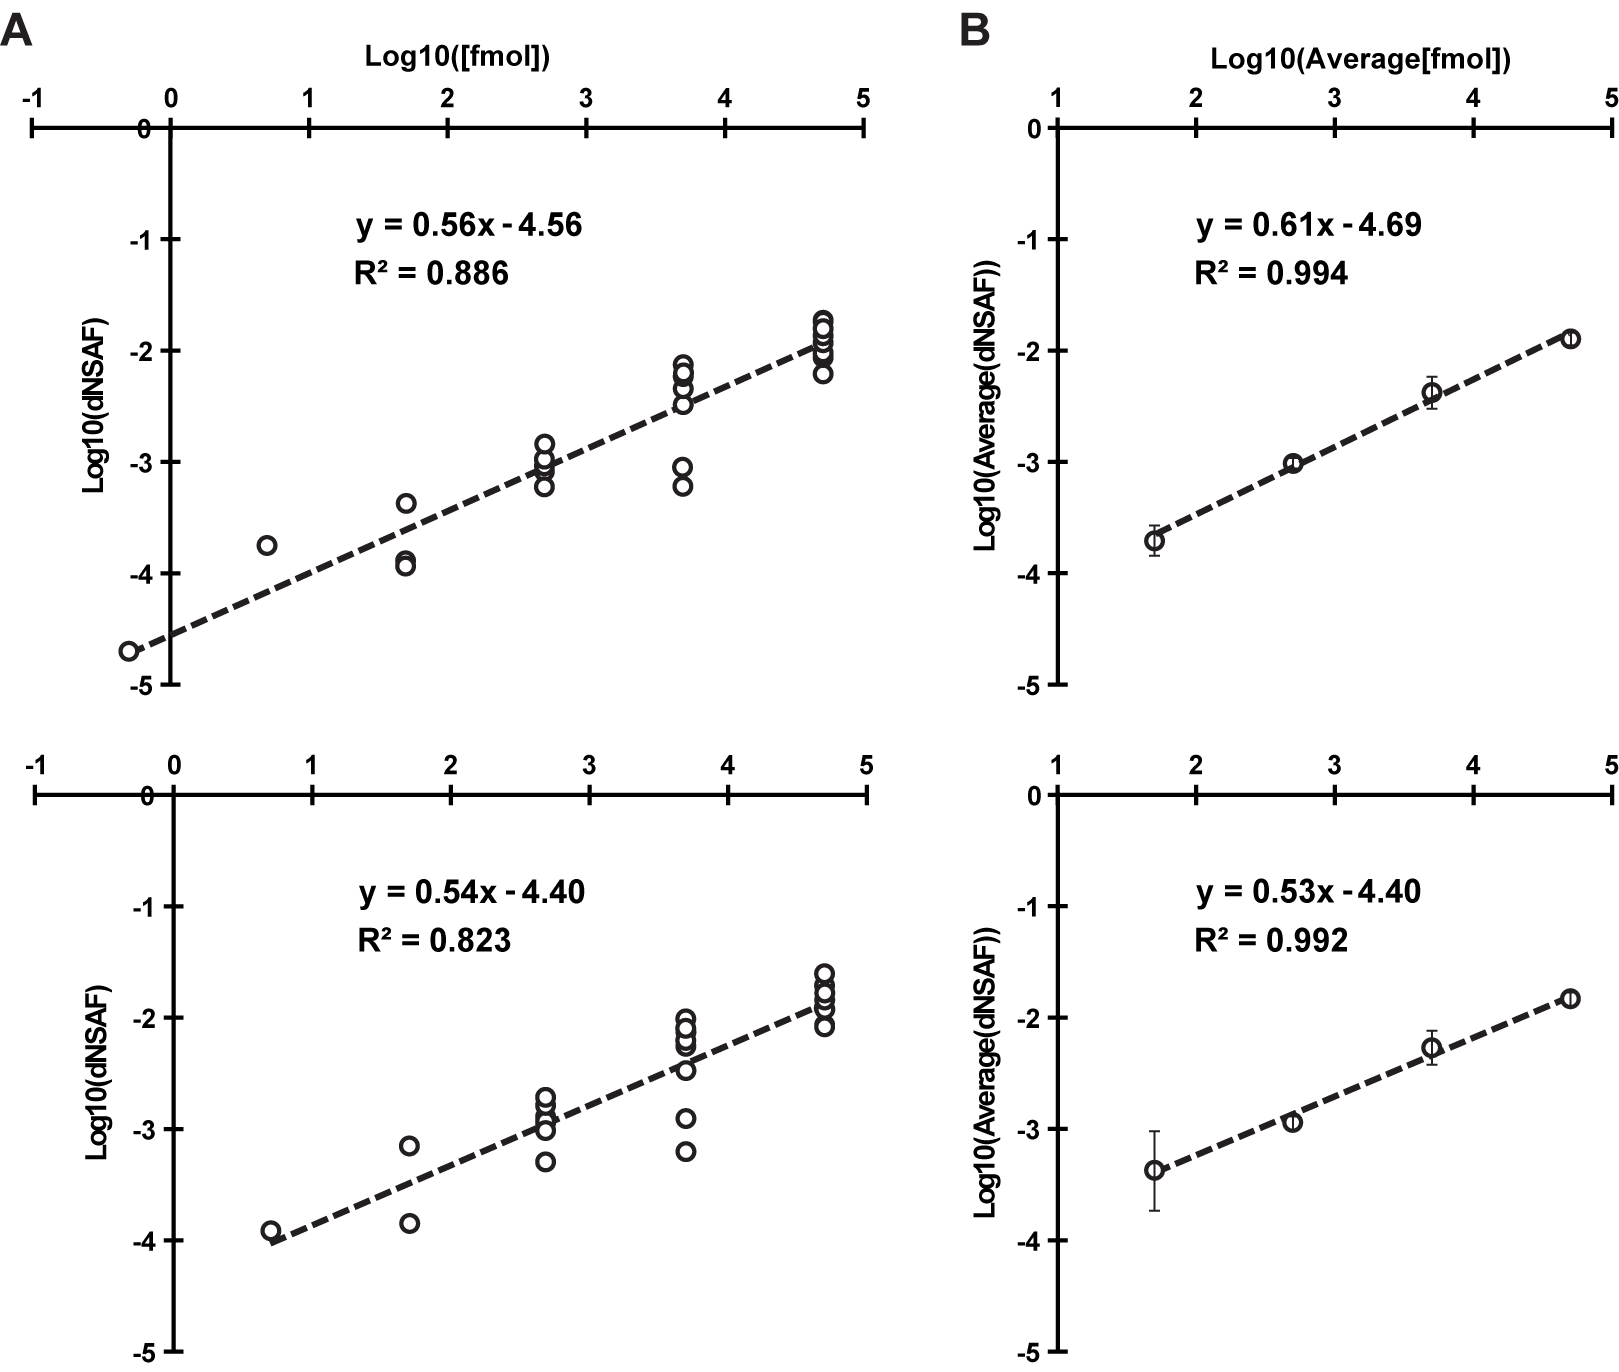
\includegraphics[width=\columnwidth]{MSpC/figure1.png}
	\mycaption{Confirmation of MSpC accuracy by analysis of MS/MS datasets generated with the Universal Proteome Standard 2 (UPS2)}{The array of UPS2 standards were spiked into Xenopus laevis egg \textbf{(Top)} and embryo \textbf{(Bottom)} extracts at a range of concentrations.  Following MS/MS analysis, dNSAF values for each protein were determined by Morpheus and MSpC.  \textbf{(A)} A log-log plot of dNSAF versus concentration for each UPS2 protein detected across each fmol range.  \textbf{(B)} A log-log plot of average dNSAF vs average concentration of each group of UPS2 proteins at each fmol range: (50, 500, 5000, and 50,000 fmol).}
	\label{fig:UPS2}
\end{figure}

Here, Xenopus egg (see top, Figure \ref{fig:UPS2}) and embryo (bottom, Figure \ref{fig:UPS2}) extracts were spiked at a 4:1 ratio with the Universal Proteome Standard 2 (UPS2), a mix of 48 purified proteins at defined molar ratios of 0.5, 5, 50, 500, 5000, and 50,000, with each ratio containing a different set of 8 of the 48 proteins.
As shown in Figure \ref{fig:UPS2} A, when the Morpheus/MSpC pipeline was used to calculate the average dNSAF value for each UPS2 protein, requiring only a single unique peptide to quantify, strong linear correlations (R$\textsuperscript{2}$ = 0.886 and 0.823) were obtained across a 1,000 fold change in abundance (50 fmol to 50,000 fmol).
In fact, the R$\textsuperscript{2}$ values were similar to those obtained by others with PSM-based LFQ methods \citep{cox14, tu14}.
This linear correlation was further strengthened when the dNSAF values were averaged for all UPS2 proteins within each of the concentration groups, with R$\textsuperscript{2}$ values of 0.994 and 0.992 for the egg and embryo datasets, respectively (see Figure \ref{fig:UPS2} B).
Notably, the slope of the concentration series was significantly less than unity, showing that NSAF measurements are not appropriate for absolute quantification, which was expected given that NSAF is a relative value.  

We also reprocessed the UPS2 dataset using the option of requiring a minimum of two unique peptides for quantification, which should improve stringency.
\begin{figure}[p]
	\centering
	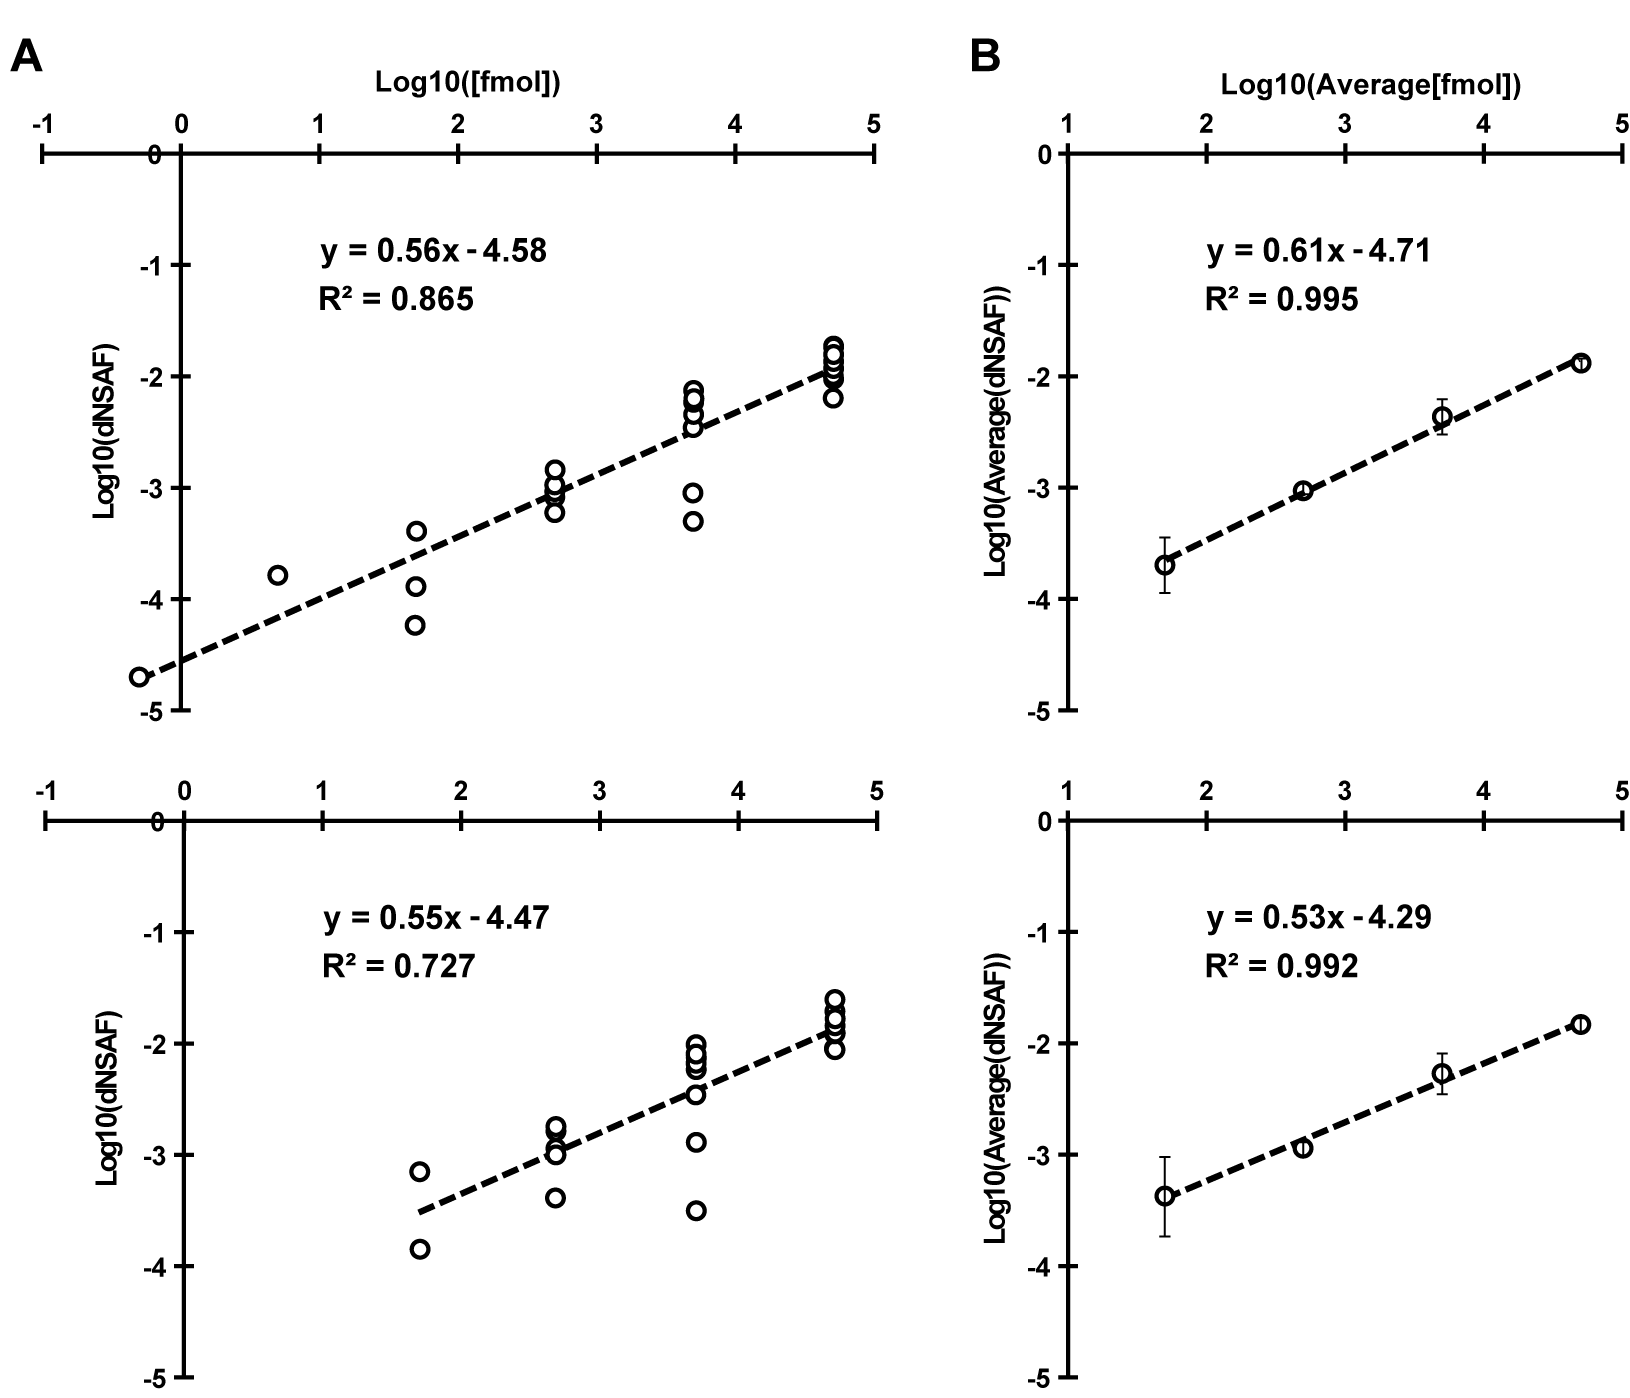
\includegraphics[width=\columnwidth]{MSpC/figure2_supplemental.png}
	\mycaption{Re- Analysis of MS/MS datasets generated with the Universal Proteome Standard 2 (UPS2)}{The array of UPS2 standards were spiked into Xenopus laevis egg \textbf{(Top)} and embryo \textbf{(Bottom)} extracts at a range of concentrations.  Following MS/MS analysis, dNSAF values for each protein were determined by Morpheus and MSpC with a change from Figure \ref{fig:UPS2} in that two unique peptides were required to quantify a protein. \textbf{(A)} A log-log plot of dNSAF versus concentration for each UPS2 protein detected across each fmol range.  \textbf{(B)} A log-log plot of average dNSAF vs average concentration of each group of UPS2 proteins at each fmol range: (50, 500, 5000, and 50,000 fmol).}
	\label{fig:UPS2twopep}
\end{figure}
This option provided only a minor improvement in overall linearity for the average UPS2 dNSAF values, but decreased linearity when each UPS2 protein was considered individually and removed some UPS2 proteins at low concentrations (compare Figure \ref{fig:UPS2twopep} A to Figure \ref{fig:UPS2} A).
Consequently, caution should be exercised when selecting this option even though it might provide a slight improvement in stringency (see Discussion on Requiring Two Peptide \ref{sec:discussiontwopep}).
To demonstrate the utility and accuracy of MSpC as applied to our work, we analyzed 20S proteasomes isolated from \textit{Arabidopsis thaliana}.
This particle contains multiple subunits assembled in stoichiometric amounts, with many subunits encoded by two paralogous genes of sufficient amino acid identity (typically >90\% \citep{yang04}) such that discrimination between paralogs can be challenging using LFQ approaches \citep{book10}.
To simulate changes in 20S proteasome abundance, we added varying amounts of trypsinized proteasomes (0.05 $\mu$g to 3 $\mu$g) to a fixed amount of trypsinized \textit{Escherichia coli} lysate (0.5 $\mu$g) to generate proteasome/lysate ratios of \textasciitilde0.091, 0.167, 0.333, 0.500, 0.667, 0.750 0.800, 0.857.
The digests were then subjected to MS/MS and the dNSAF value for each subunit along with the uNSAF value for individual isoforms were calculated by the Morpheus/MSpC pipeline (see Methods \ref{sec:methods}).
\begin{FPfigure}[Figure \ref{fig:proteasomespike} \textit{caption follows on next page}]
	\centering
	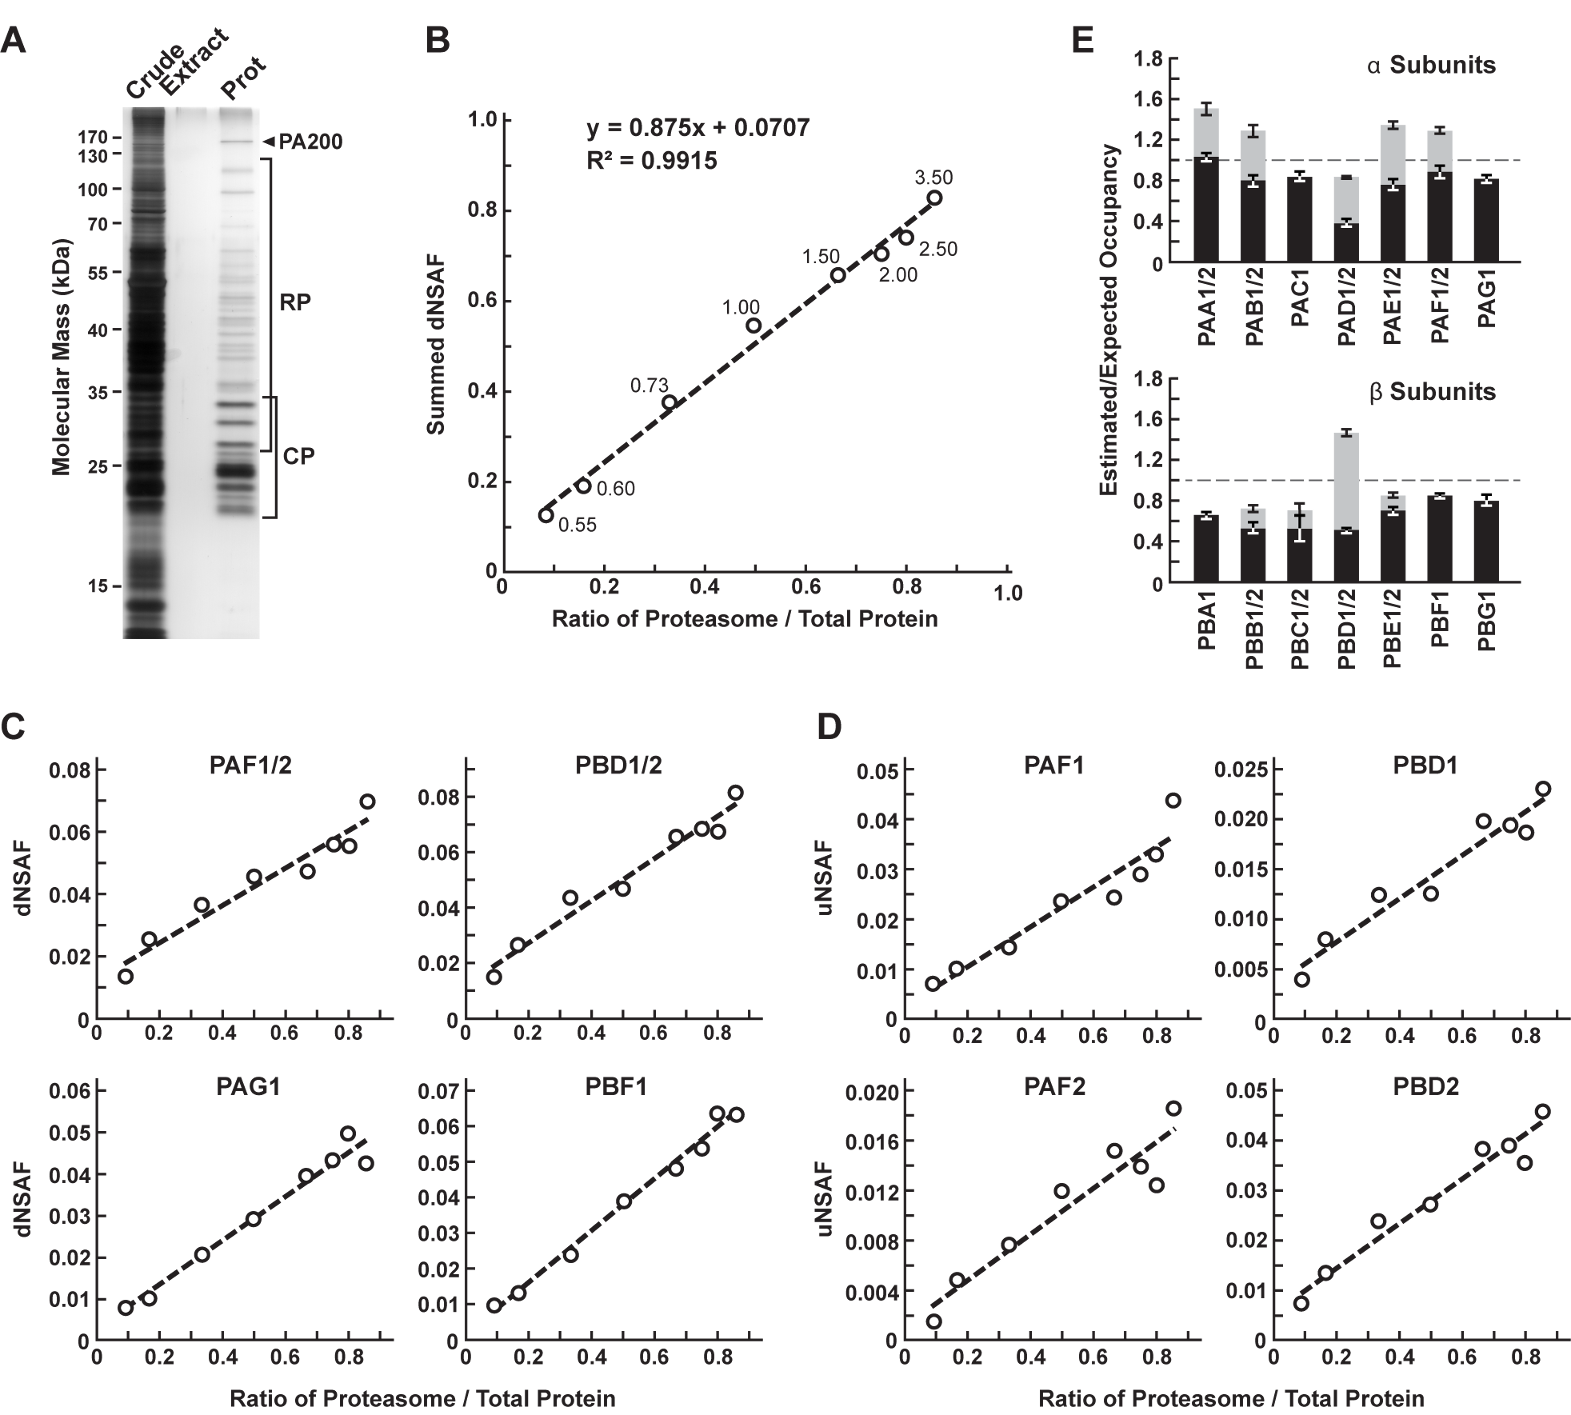
\includegraphics[width=\columnwidth]{MSpC/figure2_rescale.png}
	\mycaption{Confirmation of MSpC accuracy by analysis of MS/MS datasets generated with affinity purified \textit{Arabidopsis} 20S proteasomes spiked into a total cell lysate from \textit{E. coli}. Following MS/MS analysis, the dNSAF and uNSAF values for each subunit/isoform were determined by Morpheus and MSpC}
	{\textbf{(A)} A silver-stained SDS-PAGE gel of 20S proteasome samples affinity purified from 10-d-old \textit{Arabidopsis} seedlings. The crude seedling extract(CE), sample buffer (SB), and affinity-purified 20S proteasome samples (Prot) are shown. \textbf{(B)} Quantification of trypsinized 20S proteasomes when mixed at varying ratios with trypsinized total protein lysates from \textit{E. coli}. The spiked samples were subjected to MS/MS followed by data analysis with the Morpheus and MSpC. dNSAF values for each proteasome subunit were averaged across three technical replicates, then summed to obtain an estimate of abundance for the 20S proteasome, and plotted against their known ratios. The total protein load is listed at each point in ug. \textbf{(C} and \textbf{D)} dNSAF and uNSAF values determined from the data in panel B for individual subunits \textbf{(C)} and their isoforms \textbf{(D)} for several subunits of the 20S proteasome. \textbf{(E)} Quantification accuracy of the Morpheus/MSpC pipeline for determining the amount of each $\alpha$ and $\beta$ subunit of the 20S proteasome. SIngle subunit isoforms are in black, wheras subunits having two isoforms are shown in black and grey to reflect the contributions of isoforms 1 and 2 respectively. Each bar represents the average of eight technical replicates ($\pm$ SE). The dashed line represents the expected value of one assuming an equal stoichiometry of each subunit within the particle.}
	\label{fig:proteasomespike}
\end{FPfigure}
The data from this experiment are deposited in PRIDE with ID PXD003002.
As shown in Figure \ref{fig:proteasomespike}, MSpC provided an excellent determination for the overall abundance of 20S proteasomes within a complex mixture, along with a good reflection of the abundance of individual subunits and their isoforms.

When the dNSAF values for all subunits for the \textit{Arabidopsis} 20S proteasome including their isoforms (representing 14 distinct subunits, 10 of which exist as isoform pairs) were summed, a very close approximation of the dNSAF/actual abundance was obtained (slope=0.875) with a very strong linear correlation (R$\textsuperscript{2}$ = 0.99) over a \textasciitilde10-fold range in protein abundance.  
When each 20S proteasome subunit was analyzed individually, a strong linear response was also obtained (R$\textsuperscript{2}$ > 0.90) for a majority of subunits (Figure \ref{fig:proteasomespike} C and Table \ref{table:MSpC}).

For example, reasonably accurate concentration plots were obtained for the PAF ($\alpha$6) and PBD ($\beta$4) subunits that are encoded by the PAF1/2 and PBF1/2 gene pairs, and for the PAG ($\alpha$7) and PBF ($\beta$6) subunits that are encoded by single PAG1 and PBF1 genes (R$\textsuperscript{2}$  from 0.94 to 0.99).
Even when we calculated uNSAF values for individual isoforms added to the \textit{E. coli} lysate, strong linear responses were obtained (e.g., the PAF1/PAF2 and PBD1/PBD2 pairs) with robust correlations (R$\textsuperscript{2}$ from 0.89 to 0.95) (Figure {fig:proteasomespike} D).
Taken together, MSpC worked well for relative LFQ analysis of a multi-subunit complex and its individual subunits and isoforms within a complex proteomic mixture.

The Morpheus/MSpC pipeline also allowed us to calculate the respective incorporation of each paralog in the complex (see Isoform Incorporation Methods \ref{subsec:isoform}).
As shown in Figure \ref{fig:proteasomespike}E, these estimated/expected occupancies were close to unity for most subunits within both the $\alpha$ and $\beta$ rings of the 20S proteasome.
The only strong deviation was for PBD1/2 ($\beta$4), which  had a greater dNSAF value relative to other $\beta$ subunits across the experiments analyzed (see Table \ref{table:MSpC}).
The calculations for uNSAF values also estimated the relative proportion of each isoform within the complex for those subunits expressed from paralogous genes.
The data obtained are similar to prior studies of the complex involving quantitative top-down proteomic analysis of purified proteasome samples using ultra violet-intrinsic fluorescence to quantify tyrosine-containing subunits \citep{russell13}.
However, our MSpC analysis provided a more complete picture as several subunit isoforms were difficult to quantify by fluorescence either because they lacked tryosine, or because their fluorescence peaks overlapped with those of other subunits/isoforms.
Notably , the protein isoform ratios measured here agree well with the expression ratios for the paralogous genes \citep{book10}, suggesting that the protein isoform abundance generally reflects the relative transcriptional activity of the gene pair.
We consistently estimated slightly more $\alpha$ ring subunits (PAA-PAG) versus $\beta$ ring subunits (PBA-PBG) in the final MSpC calculations (Figure \ref{fig:proteasomespike} E).
This deviation could represent enhanced detection of $\alpha$ ring versus $\beta$ ring subunits, or more likely that purification via the tagged $\alpha$ ring subunit PAG1 also isolated assembly intermediates comprised of only $\alpha$ ring subunits.

We compared the Morpheus and MSpC pipeline to the next most comparable open source, spectral-count-based LFQ pipeline, The Trans Proteomic Pipeline (TPP) \citep{deutsch10} and ABACUS \citep{fermin11} using our datasets generated with the 20S proteasome/\textit{E. coli} lysate mixture (see Tables \ref{table:MSpC} and \ref{table:abacus}).
Morpheus/MSpC slightly outperformed TPP/ABACUS by having a greater overall accuracy (average linearity of 0.88 compared to 0.84), and by having more subunits showing an R$\textsuperscript{2}$ linear correlation greater than 0.9 (14/23 subunits for MSpC versus and 11/23 for ABACUS).
\begin{table}[h]
	\centering
	\mycaption{Table of dNSAF values for each 20S proteasome subunit generated by analyzing the proteasome spike in experiments with the Morpheus and MSpC pipeline}{The top half of the table lists $\alpha$1-7 (PAA-PAG) where 1 or 2 represent different isoforms) subunits, while the bottom half of the table lists $\beta$1-7 subunits (PBA-PBG where 1 or 2 represent different isoforms)}
\npdecimalsign{.}
\nprounddigits{2}
\begingroup
\let\clearpage\relax
\scalebox{0.7}{
\begin{tabular}{|l|l|l|l|l|l|l|l|l|l|l|}
\hline
\textbf{Ratio} & \textbf{0.091} & \textbf{0.167} & \textbf{0.333} & \textbf{0.500} & \textbf{0.667} & \textbf{0.750} & \textbf{0.800} & \textbf{0.857} &                  & \textbf{Pearsons} \\ \hline
PAA1           & 0.0102         & 0.0180         & 0.0275         & 0.0392         & 0.0505         & 0.0489         & 0.0467         & 0.0530         &                  & 0.952             \\ \hline
PAA2           & 0.0063         & 0.0072         & 0.0118         & 0.0121         & 0.0139         & 0.0218         & 0.0351         & 0.0195         &                  & 0.652             \\ \hline
PAB1           & 0.0091         & 0.0117         & 0.0209         & 0.0391         & 0.0377         & 0.0377         & 0.0268         & 0.0397         &                  & 0.721             \\ \hline
PAB2           & 0.0017         & 0.0062         & 0.0147         & 0.0223         & 0.0295         & 0.0277         & 0.0303         & 0.0250         &                  & 0.894             \\ \hline
PAC1           & 0.0076         & 0.0092         & 0.0210         & 0.0339         & 0.0373         & 0.0395         & 0.0546         & 0.0512         &                  & 0.955             \\ \hline
PAD1           & 0.0056         & 0.0070         & 0.0103         & 0.0151         & 0.0160         & 0.0147         & 0.0149         & 0.0147         &                  & 0.826             \\ \hline
PAD2           & 0.0039         & 0.0068         & 0.0141         & 0.0162         & 0.0200         & 0.0225         & 0.0255         & 0.0228         &                  & 0.959             \\ \hline
PAE1           & 0.0046         & 0.0095         & 0.0208         & 0.0352         & 0.0395         & 0.0356         & 0.0389         & 0.0490         &                  & 0.928             \\ \hline
PAE2           & 0.0063         & 0.0082         & 0.0184         & 0.0240         & 0.0269         & 0.0282         & 0.0266         & 0.0293         &                  & 0.925             \\ \hline
PAF1           & 0.0106         & 0.0173         & 0.0239         & 0.0303         & 0.0292         & 0.0379         & 0.0406         & 0.0492         &                  & 0.920             \\ \hline
PAF2           & 0.0032         & 0.0083         & 0.0128         & 0.0155         & 0.0182         & 0.0184         & 0.0152         & 0.0209         &                  & 0.847             \\ \hline
PAG1           & 0.0080         & 0.0100         & 0.0208         & 0.0291         & 0.0394         & 0.0431         & 0.0498         & 0.0423         &                  & 0.966             \\ \hline
               &                &                &                &                &                &                &                &                &                  &                   \\ \hline
\textbf{Ratio} & \textbf{0.091} & \textbf{0.167} & \textbf{0.333} & \textbf{0.500} & \textbf{0.667} & \textbf{0.750} & \textbf{0.800} & \textbf{0.857} &                  & \textbf{Pearsons} \\ \hline
PBA1           & 0.0076         & 0.0104         & 0.0170         & 0.0207         & 0.0246         & 0.0288         & 0.0337         & 0.0449         &                  & 0.898             \\ \hline
PBB1           & 0.0066         & 0.0074         & 0.0191         & 0.0276         & 0.0223         & 0.0206         & 0.0172         & 0.0227         &                  & 0.498             \\ \hline
PBB2           & 0.0009         & 0.0016         & 0.0034         & 0.0035         & 0.0110         & 0.0109         & 0.0160         & 0.0161         &                  & 0.891             \\ \hline
PBC1           & 0.0000         & 0.0000         & 0.0162         & 0.0309         & 0.0373         & 0.0344         & 0.0295         & 0.0388         &                  & 0.877             \\ \hline
PBC2           & 0.0000         & 0.0000         & 0.0000         & 0.0096         & 0.0144         & 0.0147         & 0.0146         & 0.0190         &                  & 0.931             \\ \hline
PBD1           & 0.0053         & 0.0097         & 0.0150         & 0.0147         & 0.0221         & 0.0228         & 0.0231         & 0.0271         &                  & 0.955             \\ \hline
PBD2           & 0.0094         & 0.0162         & 0.0286         & 0.0318         & 0.0426         & 0.0457         & 0.0441         & 0.0538         &                  & 0.969             \\ \hline
PBE1           & 0.0070         & 0.0097         & 0.0156         & 0.0224         & 0.0323         & 0.0373         & 0.0334         & 0.0519         &                  & 0.914             \\ \hline
PBE2           & 0.0007         & 0.0003         & 0.0036         & 0.0069         & 0.0080         & 0.0105         & 0.0106         & 0.0133         &                  & 0.973             \\ \hline
PBF1           & 0.0093         & 0.0122         & 0.0205         & 0.0310         & 0.0368         & 0.0412         & 0.0473         & 0.0459         &                  & 0.991             \\ \hline
PBG1           & 0.0085         & 0.0165         & 0.0203         & 0.0323         & 0.0331         & 0.0345         & 0.0334         & 0.0442         &                  & 0.912             \\ \hline
               &                &                &                &                &                &                &                &                &                  &                   \\ \hline
               &                &                &                &                &                &                &                &                & \textbf{Average} & \textbf{0.885}    \\ \hline
\end{tabular}

}
\endgroup
\npnoround
\label{table:MSpC}
\end{table}
\begin{table}[h]
	\centering
	\mycaption{Table of adj\_NSAF values for each 20S proteasome subunit (equivalent to dNSAF) generated by analzying the proteasome spike in experiments with the TPP and ABACUS pipeline}{The top half of the table lists $\alpha$1-7 (PAA-PAG) where 1 or 2 represent different isoforms) subunits, while the bottom half of the table lists $\beta$1-7 subunits (PBA-PBG where 1 or 2 represent different isoforms)}
\npdecimalsign{.}
\nprounddigits{2}
\begingroup
\let\clearpage\relax
\scalebox{0.7}{
\begin{tabular}{|l|l|l|l|l|l|l|l|l|l|l|}
\hline
\textbf{Ratio} & \textbf{0.091} & \textbf{0.167} & \textbf{0.333} & \textbf{0.500} & \textbf{0.667} & \textbf{0.750} & \textbf{0.800} & \textbf{0.857} &                  & \textbf{Pearsons} \\ \hline
PAA1           & 125.16         & 166.81         & 245.61         & 355.60         & 491.76         & 494.18         & 504.75         & 554.97         &                  & 0.988             \\ \hline
PAA2           & 57.52          & 70.52          & 114.60         & 126.35         & 132.06         & 162.25         & 358.13         & 154.62         &                  & 0.493             \\ \hline
PAB1           & 96.13          & 134.98         & 207.90         & 328.16         & 362.21         & 416.46         & 303.60         & 397.39         &                  & 0.865             \\ \hline
PAB2           & 29.67          & 79.42          & 153.34         & 282.91         & 365.22         & 299.47         & 310.19         & 299.93         &                  & 0.849             \\ \hline
PAC1           & 95.27          & 112.45         & 214.24         & 376.66         & 389.05         & 361.39         & 512.73         & 488.62         &                  & 0.925             \\ \hline
PAD1           & 62.58          & 76.16          & 106.03         & 196.03         & 179.37         & 182.99         & 164.04         & 188.71         &                  & 0.794             \\ \hline
PAD2           & 39.88          & 68.33          & 145.34         & 178.43         & 190.84         & 246.20         & 243.28         & 240.01         &                  & 0.954             \\ \hline
PAE1           & 50.41          & 97.53          & 193.18         & 368.87         & 464.79         & 397.27         & 468.64         & 534.16         &                  & 0.951             \\ \hline
PAE2           & 71.38          & 80.07          & 184.85         & 255.98         & 299.41         & 290.16         & 304.77         & 348.32         &                  & 0.955             \\ \hline
PAF1           & 132.67         & 179.60         & 207.68         & 253.51         & 253.04         & 327.11         & 334.73         & 460.76         &                  & 0.835             \\ \hline
PAF2           & 0.00           & 0.00           & 59.62          & 70.93          & 111.83         & 80.29          & 63.08          & 65.86          &                  & 0.606             \\ \hline
PAG1           & 108.09         & 142.82         & 271.18         & 389.94         & 495.94         & 530.90         & 632.72         & 540.86         &                  & 0.966             \\ \hline
               &                &                &                &                &                &                &                &                &                  &                   \\ \hline
\textbf{Ratio} & \textbf{0.091} & \textbf{0.167} & \textbf{0.333} & \textbf{0.500} & \textbf{0.667} & \textbf{0.750} & \textbf{0.800} & \textbf{0.857} &                  & \textbf{Pearsons} \\ \hline
PBA1           & 85.99          & 113.01         & 208.38         & 233.44         & 273.50         & 327.23         & 417.12         & 560.62         &                  & 0.851             \\ \hline
PBB1           & 47.77          & 80.66          & 195.35         & 324.53         & 303.26         & 220.36         & 200.51         & 216.77         &                  & 0.440             \\ \hline
PBB2           & 17.11          & 4.54           & 0.00           & 0.00           & 21.05          & 102.51         & 144.30         & 187.86         &                  & 0.618             \\ \hline
PBC1           & 27.19          & 40.65          & 165.46         & 345.14         & 364.19         & 386.59         & 338.47         & 373.16         &                  & 0.885             \\ \hline
PBC2           & 10.64          & 40.65          & 0.00           & 55.58          & 145.43         & 158.90         & 159.74         & 228.05         &                  & 0.845             \\ \hline
PBD1           & 50.14          & 94.46          & 168.58         & 167.50         & 244.25         & 248.17         & 252.65         & 319.61         &                  & 0.945             \\ \hline
PBD2           & 81.45          & 149.28         & 256.88         & 319.89         & 390.60         & 407.02         & 380.30         & 490.17         &                  & 0.950             \\ \hline
PBE1           & 81.01          & 107.76         & 196.21         & 302.90         & 365.03         & 404.25         & 378.67         & 441.03         &                  & 0.981             \\ \hline
PBE2           & 0.00           & 1.52           & 5.59           & 8.05           & 40.06          & 56.56          & 59.39          & 58.56          &                  & 0.887             \\ \hline
PBF1           & 71.53          & 112.26         & 190.45         & 226.89         & 259.90         & 366.60         & 431.42         & 420.23         &                  & 0.943             \\ \hline
PBG1           & 104.93         & 174.55         & 232.34         & 392.37         & 425.10         & 397.85         & 396.42         & 463.13         &                  & 0.906             \\ \hline
               &                &                &                &                &                &                &                &                &                  &                   \\ \hline
               &                &                &                &                &                &                &                &                & \textbf{Average} & \textbf{0.845}    \\ \hline
\end{tabular}
}
\endgroup
\npnoround
\label{table:abacus}
\end{table}

In addition to this modest improvement, we note that the Morpheus/MSpC pipeline required significantly less intermediary steps, thus accelerating the data analysis.
Some of the additional steps in TPP/ABACUS could be automated from the command-line, but it would likely be a challenge for the average user.
Importantly, we found that the Morpheus/MSpC pipeline was faster.
Timing tests using the proteasome/\textit{E. coli} spike data generated here showed that the Morpheus/MSpC pipeline was 1.9-fold faster than the TPP/ABACUS pipeline (Figure \ref{fig:MSpCspeed}).
Such an improvement was expected given that Morpheus completes its searches on average 1.3 to 4.6 times faster than most other search engines available \citep{wenger13}. 
Given its simplicity of use, speed, and open source nature, MSpC combined with Morpheus is clearly advantageous over other PSM-based LFQ approaches currently available.  Moreover, by being open source, MSpC should allow others to extend its utility and to serve as a platform for integrating additional open source LFQ approaches into the Morpheus pipeline. 

\begin{figure}[p]
	\centering
	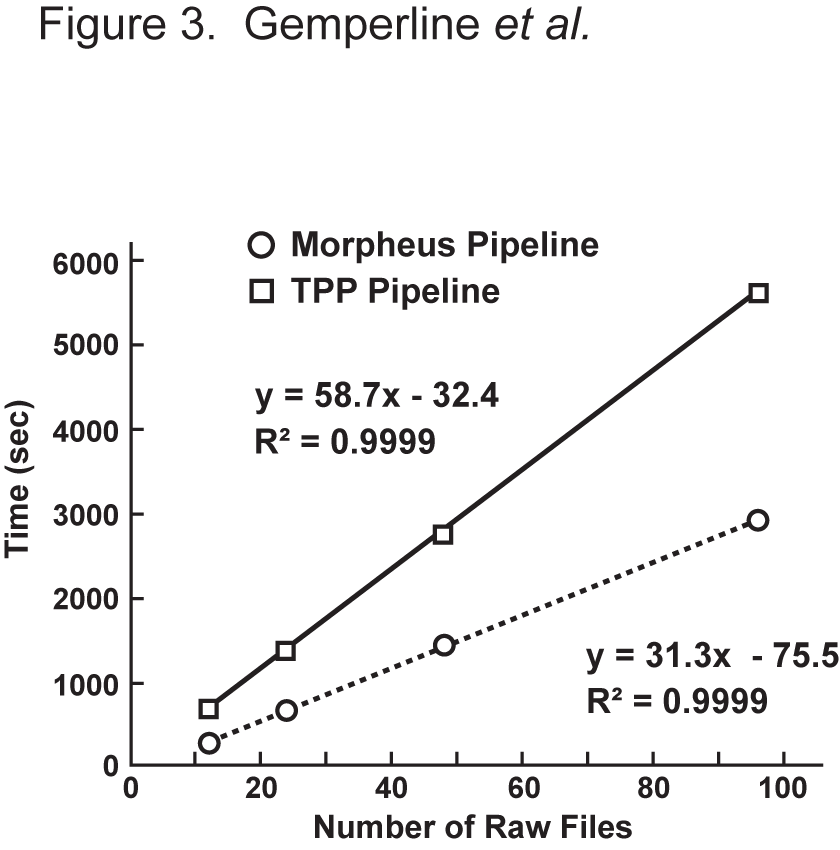
\includegraphics[width=\columnwidth]{MSpC/figure3.png}
	\mycaption{MSpC combined with Morpheus works faster than TPP combined with ABACUS.  Speed comparisons were performed for 12, 24, 48, and 96 raw MS/MS files generated with the 20S proteasome/\textit{E. coli} lysate samples analyzed in \ref{fig:proteasomespike}}{On average, Morpheus/MSpC finished the calculations 1.9 times faster than TPP/ABACUS over a \textasciitilde10-fold range of dataset size.}
	\label{fig:MSpCspeed}
\end{figure}

\section {Methods}
\label{sec:methods}
\subsection{Sample Preparation}

All chemicals were purchased from Sigma-Aldrich unless otherwise stated.  20S proteasomes were obtained as described previously \citep{book10} from \textit{Arabidopsis thaliana} Col-0 ecotype seedlings in which the 20S proteasome subunit PAG1 ($\alpha$7) was genetically replaced with a FLAG-tagged variant, with the minor modification of switching to a more stable HEPES buffer during purification.  The FLAG peptide used for elution was removed by filtering through an Amicon Ultra 4 10K filter with the elution buffer also exchanged into 8 M urea.  Total protein was quantified by the bicinchoninic acid protein assay (Thermo Scientific) using bovine serum albumin as the standard.  Approximately 70 $\mu$g of proteasomes were digested overnight at 37$^\circ$C using a 1:30 trypsin/sample ratio.  Peptides were acidified to a final concentration of 1\% TFA, desalted on a Waters C18 Sep-Pak containing 50 mg sorbent material, and lyophilized.  Total \textit{E coli} lysates were obtained from Bio-Rad (Cat. 163-2110) with 200 $\mu$g digested as above.  Both proteasome and \textit{E. coli} peptides were dissolved in 5\% acetonitrile, 95\% water, and 0.1 \% formic acid.  Each MS analysis, performed in triplicae, used 5 $\mu$L volumes prepared with 3, 2, 1.5, 1, 0.5, 0.25, 0.1, or 0.05 $\mu$g of digested proteasomes mixed with 0.5 $\mu$g of digested E. c.oli proteins.  This mixtures reflected proteasome/\textit{E. coli} ratios of \textasciitilde0.091, 0.167, 0.333, 0.500, 0.667, 0.750 0.800, and 0.857, respectively.

\subsection{Liquid Chromatography and High-Resolution Mass Spectrometry}

Samples were analyzed by ultra-high performance liquid chromatography (UPLC) (nanoAcquity, Waters Corporation) connected online to an electrospray ionization LTQ Velos Orbitrap mass spectrometer (Thermo Scientific).  Separation employed a 100 x 365 $\mu$m fused silica capillary micro-column packed with 20 cm of 1.7 $\mu$m-diameter, 130-$\AA$ pore size, C18 beads (Waters BEH), with an emitter tip pulled to approximately 1 $\mu$m using a laser puller (Sutter Instruments).  Peptides were loaded at a flow-rate of 400 nL/min for 30 min and then eluted over 120 min at a flow-rate of 300 nL/min with a 2\% to 30\% acetonitrile gradient in 0.1\% formic acid.  Full-mass scans were performed in the FT Orbitrap with a mass range of 300-1500 m/z at a resolution of 60,000, followed by ten MS/MS high energy C-trap dissociation scans of the ten highest intensity parent ions at 42\% normalized collision energy and 7,500 resolution, with a mass range starting at 100 m/z.  Dynamic exclusion was enabled with a repeat count of two over the duration of 30 sec and an exclusion window of 120 sec.  

\subsection{Data Processing}

Protein identifications were determined using the Morpheus search engine \citep{wenger13}.  Raw data was searched with the Thermo module of Morpheus revision 151 downloaded and compiled from source code available at \url{http://sourceforge.net/projects/morpheus-ms/} using Microsoft Visual Studio 2013 professional edition.  The following parameters were used to search all databases: unknown precursor charge states - +2, +3, +4; maximum number of MS/MS peaks = 400; assign charge states - enabled; de-isotope - disabled; generate target decoy database on the fly; protease trypsin (no proline rule); maximum missed cleavages = 2; initiator methionine behavior - variable; fixed modification of carbamidomethylation of cysteine; variable modification of oxidation of methionine; maximum variable modification isoforms per peptide = 1024; precursor mass tolerance = $\pm$ 2.1 Da monoisotopic (recommended parameters to account for neutral loss); precursor monoisotopic peak correction - disabled; product mass tolerance = $\pm$ 0.025 Da monoisotopic; consider modified forms as unique peptides - false; maximum threads = 8; minimize memory usage - false.   
MSpC quantification of Universal Proteome Standard 2 (UPS2) protein sequences exploited the MS/MS analysis of individual USP2 proteins (Sigma-Aldrich) mixed at various concentrations with egg or embryo extracts from Xenopus laevis available in the PRoteomics IDEntifications (PRIDE) repository \citep{vizcaino13} using identifier - PXD000902 and the available proteomics database - pita\_v1.71.protein.name.fa.  For our analysis, both the raw MS/MS data and resulting FASTA files for the USP2 and egg and embryo proteomes were obtained from PRIDE.  The database used for searching the MS/MS data of \textit{Arabidopsis} proteasomes spiked into total \textit{E. coli} peptides was generated by combining Uniprot K12 \textit{E. coli} reference proteome UP000000625 with a common contaminant database, and then mixing the merged dataset with FASTA sequences for all proteoforms of all known proteasome subunits and associated proteins \citep{book10} obtained from the TAIR10\_pep\_20101214 FASTA database available within The \textit{Arabidopsis} Information Resource (TAIR) version 10.  All FASTA files are available for download in the Supporting Information.  The datasets were analyzed by MSpC with a 1\% PSM false discovery rate (FDR) and a 1\% protein group FDR to determine NSAF, dNSAF, and uNSAF values for each protein group. Two separate analyses were performed in which one unique, or alternatively two unique peptides were required to quantify a protein group.  NSAF values were calculated according to formulas 1a, 2a, and 3a from Figure 1 of Zhang et al. \citep{zhang10}.

\subsection {Isoform Incorporation Rates}
\label{subsec:isoform}
	For the individual subunit analysis of the 20S proteasome the isoform incorporation rates were treated as follows. Given that each proteasome subunit should be incorporated at equal stoichiometry within the 20S particle, we then tested whether the Morpheus/MSpC pipeline could calculate the relative abundance of each subunit and the distribution of isoforms.  Here, we divided the dNSAF values for each subunit/isoform by the total number of dNSAF values for the entire complex across all eight total proteasome/\textit{E. coli} lysate ratios tested.  This averaged value provided a concentration-independent ratio for the incorporation of each subunit/isoform.  We then normalized these values based on a 1/14 stoichiometry of each subunit within the complex to calculate the estimated occupancy versus the expected occupancy of each subunit.  

\subsection{Speed and Accuracy Comparisons of Morpheus/MSpC to the TPP/ABACUS Pipeline}

The speed and accuracy of MSpC combined with Morpheus was compared to the next most comparable open source software suite for calculating NSAF values; i.e., TPP \citep{deutsch10} combined with ABACUS \citep{fermin11}, using the proteasome spike-in experiment files as input.  The .raw files were converted to .mzmL files by TPP Build 201411201551-6764 and then searched using the multi-threaded X!Tandem MS/MS search engine \citep{craig04} with the search parameters adjusted as close as possible to that used for the Morpheus searches.  A decoy database was generated using the TPP tool DecoyFASTA for use with X!Tandem.  Relevant  X!Tandem parameters are listed here: parent monoisotopic mass error = $\pm$ 2.1 Da, fragment mass error = $\pm$ 0.025 Da, fixed modifications of carbamidomethylation (57.021464) on cysteine, and variable modification of oxidation (15.994915) on methionine, fully tryptic cleavages, missed cleavage sites = 2 maximum, no refinement and 8 threads.  The configuration file used and the test datasets can be found in the Supporting Information. The data were analyzed in the TPP using Peptide Prophet \citep{keller02}.  Relevant settings are listed: minimum probability = 0.05; minimum peptide length = 7; accurate mass, and nonparametric decoy database to pin down false discovery rate; ignore +1 charged spectra; and run Protein Prophet \citep{nesvizhskii03} after Peptide Prophet.  
Once completed, all pepxml data from Peptide Prophet contained in a single folder was combined using the command line version of Protein Prophet from the TPP binaries with the following command: ProteinProphet.exe *.pep.xml interact-COMBINED.prot.xml.  This post-analysis aggregation was required for running the spectral counting program ABACUS.  Here, we note that there are no graphic user interfaces to perform this post analysis aggregation, which makes this portion of the data analysis more difficult for those unfamiliar with setting up and running programs from the command line.  The combined data was analyzed by ABACUS with the following parameters: best peptide probability = 0.99; minimum peptide probability = 0.99; experimental peptide probability = 0; and combined file probability = 0.99 to most accurately match a 1\% FDR stringency settings in MSpC.  dNSAF values were compared in Microsoft Excel using the CORREL function and squaring the result.  Additional timing tests were performed with a subset of the calibration curve data (ratios 0.091, 0.167, 0.333, and 0.500 in triplicate corresponding to 12 .raw files) by increasing file input to 24 (2x), 48 (4x), and 96 (8x) .raw files to determine the time dependence on input size between both pipelines tested (Morpheus/MSpC versus TPP/ABACUS).  The timing tests and all data analyses were performed on a computer running Windows 7 Ultimate, with 16 GB of random access memory, and an Intel Core i7-2700k with hyper-threading turned on for eight logical cores.

\section {Discussion on Requiring Two Unique Peptides to Quantify a Protein}
\label{sec:discussiontwopep}
Occasionally, some researchers may want to use a more stringent criterion for quantification such as requiring a protein to have more than one unique identifying peptide. To see how this might affect our data analysis, we re-analyzed our results shown in Figure \ref{fig:UPS2twopep}, this time requiring two unique peptides to quantify an individual protein. The results point to a very small increase in linearity observed in the average plots; however, there is a slight decrease in linearity for the egg sample (0.886 to 0.865) and a larger decrease in linearity for the individual UPS2 protein plot for the embryo sample (0.827 to 0.723). The decrease in linearity in the embryo sample is due to the analysis removing a low abundance UPS2 protein (O00762ups) identified with only one unique peptide. While some have suggested that requiring more than one unique peptide to identify a protein is an ideal approach, requiring two peptides for identifications in database searches reduces the number of protein identifications in the target database more than those in the decoy database and results in increased false discovery rates . While we recognize that researchers may want to implement more stringent requirements than what is typically used in database searching to quantify a set of proteins, there are two cases where requiring two unique peptides may not be ideal in a quantitative analysis. Firstly, low abundance proteins that have few PSMs might be identified by only a single peptide and thus be erroneously thrown out of the analysis. Secondly, there may be only one unique peptide that can differentiate between families of homologous proteins. In this second case, requiring two unique peptides would remove these homologous proteins from the MSpC analysis, even if they had a large number of PSMs. Because of these reasons and because of the decreased linearity observed when requiring proteins to have two unique peptides (Figure \ref{fig:UPS2twopep}) as compared to one unique peptide (Figure \ref{fig:UPS2}), we suggest caution in requiring more than one unique peptide per protein.

\section {Tutorial}
\label{sec:tutorial}

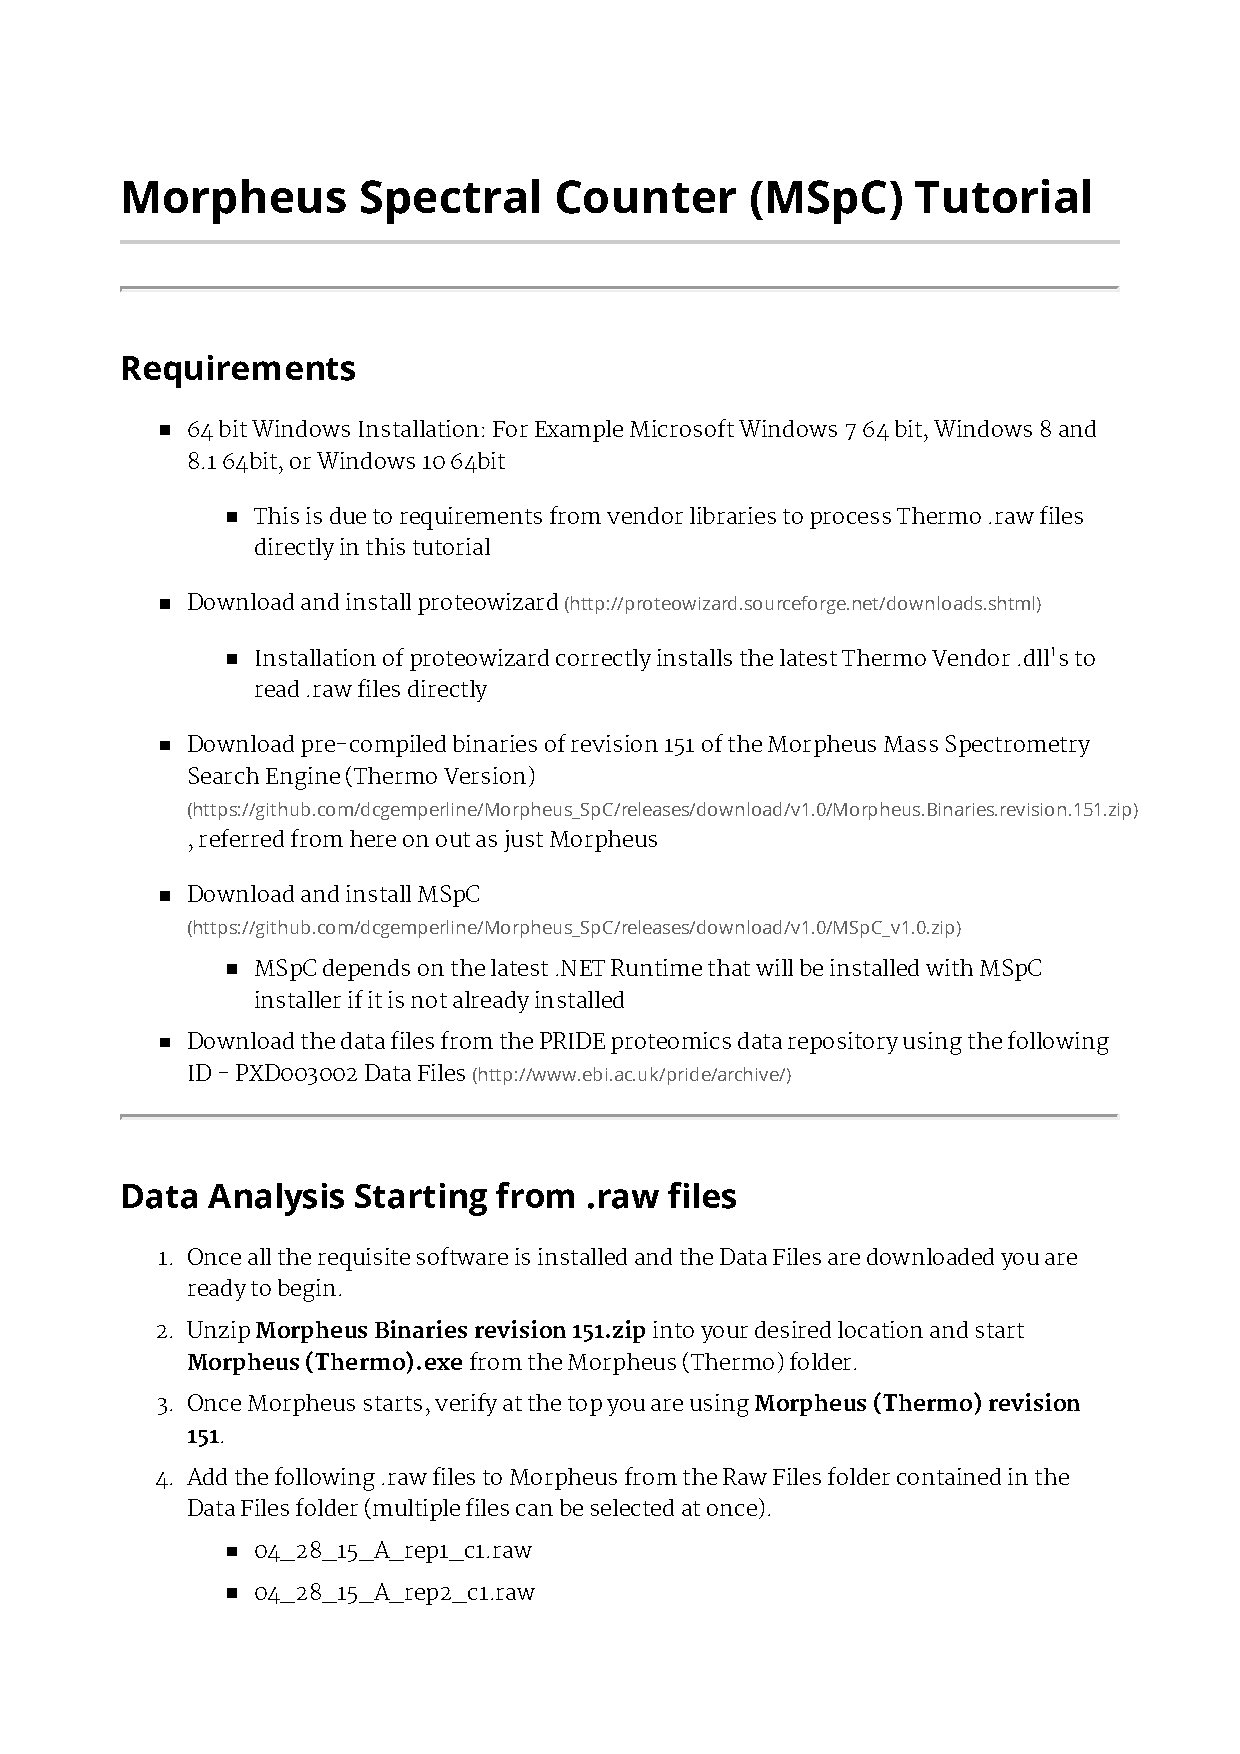
\includepdf[pages=-]{MSpC/Tutorial.pdf}


\section {Acknowledgements}
D.C.G. was supported by a grant from the U.S. Department of Energy Office of Science; Office of Basic Energy Sciences; Chemical Sciences, Geosciences, and Biosciences Division (DE-FG02-88ER13968) and a graduate training fellowship from the NIH (5 T32 GM 7133-37).  M.S. and L.M.S were supported by a grant from the National Institute of Health/National Institute of General Medical Sciences (1P50HG004942).  The authors thank Erin Gemperline, Richard S. Marshall, and Josh Coon for critical reading of the manuscript, and additionally thank Derek Bailey for a critical code review.

\begin{singlespace}
\bibliographystyle{plant_cell_final}
\renewcommand\bibname{Literature Cited}
\bibliography{MSpC}
\end{singlespace}

\chapter{Identifying Core Protease and Regulatory Particle Specific Interactors}

\section{Summary}

\section{Introduction}

\section{Experimental Procedures}

\section{Results}

\section{Discussion}

\section{Conclusions}


% \include{motivation/motivation}
% \include{related/related}

%% etc, etc.

%% Do you have appendices?  If so, add them here, just like chapters.
% \begin{appendices}
% \include{backmatter/appendix1}
% \end{appendices}

%% Are you a big nerd with a colophon?  Add it here.
\begin{colophon}
This document was typeset with \LaTeX \ . It is based on the University of Wisconsin dissertation template created by William C. Benton (available at \url{https://github.com/willb/wi-thesis-template}).
 

\end{colophon}

%% McBride is a very nice style (some version is included in this distribution)
%\bibliographystyle{mcbride}
%\bibliography{your-bib-file}

%% Want an index?  Neither did I.
%\printindex

\end{document}
